\documentclass[11pt,a4paper]{report}
\usepackage[a4paper,bindingoffset=0.2in,%
	left=1.25in,right=0.75in,top=1.25in,bottom=1in,%
	footskip=.25in]{geometry}
\usepackage{graphicx}
\usepackage{blindtext}
\usepackage{mhchem} % for chemical equation, e.g.: \ce{MgSO4}
\usepackage[super]{nth}

\usepackage{xcolor} %for making colored texts; List of predefined color: black, blue, brown, cyan, darkgray, gray, green, lightgray, lime, magenta, olive, orange, pink, purple, red, teal, violet, white, yellow

\usepackage{enumitem}
\usepackage{nicefrac} % for fraction in an equation
\usepackage{xfrac} % for fraction in an equation
\usepackage{mathtools} % only for \binom
\usepackage{amsmath}
\usepackage{amssymb}
%\usetikzlibrary{shapes.geometric, arrows}
\usepackage{booktabs}

\usepackage[right]{lineno}	% line numbers
\usepackage{siunitx}
\usepackage{fancyhdr}
\usepackage{cite} % citation
\usepackage{listings} % for listing commands

\pagestyle{fancy}
\fancyhf{}
%\fancyhead[R]{\slshape \rightmark}
\fancyhead[L]{\slshape \leftmark}
\fancyhead[R]{\color{red}\textit{(Draft)}}
%\lhead{\textit{ICU Protocol {\color{red}(Draft)}}}
%\rhead{\textit{icddr,b Dhaka Hospital}}
\renewcommand{\headrulewidth}{0.4pt}


%\fancyfoot[L]{Draft}
\fancyfoot[R]{Page $|$ \thepage}
%\rfoot{Page $|$ \thepage}
\renewcommand{\footrulewidth}{0.4pt}

\usepackage{tikz}
\usetikzlibrary{scopes}

\usepackage{imakeidx}
%\makeindex
\makeindex[columns=3, title=Index, intoc]
\usepackage[hidelinks]{hyperref}
%\makeindex[columns=3, title=Alphabetical Index, intoc]

\usepackage{multirow}



%===============================
%	BODY OF THE DOCUMENT 
%===============================

\begin{document}
\setcounter{secnumdepth}{3}
\setcounter{tocdepth}{1}
%\linenumbers

%==========================
%	TITLE PAGE 
%==========================
\begin{titlepage}
	\centering 
	~\\
	\vspace{1.5cm}
	
	\includegraphics[scale=0.30]{icddrb.png}
	%	\label{icddrb_logo}
	
	\vspace{2.0cm}
	{\color[rgb]{0.0,0.0,.55}{\Huge\textbf{The Handbook of}}} \\
	\vspace{3mm}
	{\color[rgb]{0.0,0.0,.55}{\Huge\textbf{icddr,b Dhaka Hospital}}} \\
	\vspace{3mm}
	\textit{\nth{4} edition; June, 2018}
	%	{\Huge\textbf{Management protocol in ICU, \\ icddr,b Dhaka Hospital}}
	
	\vspace{1.5cm}
	\textbf{{\color{red}( FINAL DRAFT )}}

	
	\vspace{1.5cm}
	{\Large icddr,b: Centre for Health and Population Research} \\
	GPO Box 128 \\
	Dhaka 1000, Bangladesh 
	
	\vspace{1.75cm}
{\large \textit{Approved by}} {\color{red}(pending)} \\
	{\large Dr. Mohammod Jobayer Chisti, Senior Scientist}

\vspace{5.00mm}
{\large \textit{Reviewed by}} \\
	{\large Dr. Farzana Afroze}, Senior Medical Officer \\
	{\large Dr. Monira Sarmin}, Medical Officer \\

\vspace{5.00mm}
{\large \textit{Prepared by}} \\
	{\large Dr. Visnu Pritom Chowdhury}, Clinical fellow \\
	\href{mailto:pr3370m@gmail.com}{\texttt{visnu.pritom@icddrb.org}}
\end{titlepage}

\tableofcontents
\listoffigures
\listoftables


\newpage
\clearpage
\begin{flushright}
	\thispagestyle{empty}
	\vspace*{\fill}
	\textit{Dedicated to, }\\ 
	\vspace{7.0mm}
	\textbf{\textit{ \fontsize{15}{1}\selectfont My fellow colleagues at icddr,b}}\\ 
	\vspace{5.00mm}
	\textit{Hope it helps}
	\vspace*{\fill}
\end{flushright}
\clearpage

%============================================
% CHAPTER: WHEN A PATIENT COMES TO ICU
%============================================
\chapter[General approach]{General approach to a critically ill patient}


%============================================
%	INITIAL ASSESSMENT
%============================================
\section[Initial assessment]{Initial assessment $\rightarrow$ follow ABCDE}
Check the followings:

\begin{enumerate}[noitemsep]
	\item \textbf{A} ppearance of the patient; such as, lethargic, gasping, having convulsion, rolling of eyeball, staring and such
	\item \textbf{B} reathing: Respiratory status (airway obstruction: suction, hypoxia: \ce{O2} support)
	\item \textbf{C} irculation: Check pulse, BP, CRT, temperature and RBS
	\item \textbf{D} ehydration status 
	\item \textbf{E} lse: 
	\begin{enumerate}
		\item Abdominal distension, or any signs of electrolyte imbalance 
		\item Urine output, or, any history of taking concentrated ORS
		\item In case of adult patient, check BP and CVP; consider an ECG as well
		\item Look for other signs; for examples, 
		\begin{itemize}[noitemsep]
			\item Pupilary reaction, jerks, planter response, features of meningism
		\end{itemize}
		\item For elderly patients ask for chronic diseases and drug history, especially steroid. 
	\end{enumerate}
\end{enumerate}


%============================
%	MANAGEMENT OUTLINE
%============================
\section{Management outline}
During assessment of nutritional status, please consider dehydration status. If a baby has some dehydration please add an extra 5--7.5\% weight (equivalent to weight loss in some dehydration) with the measured weight to determine precise nutritional status. 

\subsection{Antibiotic}
Please see the dedicated chapter/s. 

\subsection{Micronutrient}
(for chisldren with SAM)

\begin{enumerate}
	\item Inj. \ce{MgSO4}: 0.1 ml/kg/day, for 5 -- 7 days (IM)
	\item Tab. Folic acid: 1.25 mg, once daily, for 10 days 
	\item Tab. Zinc 20 mg: 1 tablet, once daily, for 10 days (age \textgreater 6 months) \\ \sfrac{1}{2} tab if age $\geq$2 months but $<$6 months 
	\item Cap. Vitamin A: 
	\begin{itemize}[noitemsep]
		\item 2 months -- $<$6 months\hspace{3mm}: \hspace{2mm}50,000 IU, Stat
		\item 6 months -- $<$12 months : 100,000 IU, Stat
		\item 12 months -- 5 years\hspace{8mm}: 200,000 IU, Stat
	\end{itemize}
	{\color{red}$\star$} If measles, another dose on 2nd day \\
	{\color{red}$\star$} For eye changes due to malnutrition, on day 1, 2 and 14
	
	\item Multivitamin drops:
	\begin{itemize}[noitemsep]
		\item Age $<$1 year: 0.5 ml, 12 hourly, for 10 -- 15 days 
		\item Age $\geq$1 year: 1 ml, 12 hourly, for 10 -- 15 days 
	\end{itemize}
	\item Syr. Potassium Chloride (KCl): 4 mmol/kg/day, in 3 divided dosage, for 3 -- 5 days (1 TSF = 7 mmol/l)\\
	{\color{red}$\bullet$} for quick dispense, $\approx$1 ml/kg
\end{enumerate}



%========================
%	COMPLICATIONS
%========================
\subsection{Complications}
\begin{enumerate}
	\item \textbf{Hypoglycemia\index{Hypoglycemia}}: 10\% glucose, 5 ml/kg, IV Stat \& \\ 10\% glucose 50 ml orally; 25 ml for infant.\\ \\
	\textbf{Correction of repeated $\downarrow\downarrow$glycemia correction in children} \\
	Look for features of infection. 
	\begin{itemize}
		\item Symptomatic child
		\begin{itemize}
			\item IV 10\% glucose 
			\item $+$ hourly glucose 
			\item Hourly diet
		\end{itemize}
		\item Asymptomatic child 
		\begin{itemize}
			\item Oral 10\% glucose 
			\item $+$ hourly diet
		\end{itemize}
		\item If $\geq$2 episodes of hypoglycemia
		\begin{itemize}
			\item Send to ICU
			\item Give correction
			\item Repeat RBS 30 minutes later
		\end{itemize}
	\end{itemize}
	
	~\\
	\textbf{In ICU}: 
	\noindent i.e. \nth{3} episode: \\
	IV + Oral correction $\rightarrow$ \sfrac{1}{2} oral diet, hourly + \sfrac{1}{2} IV (with 5\% dextrose @3ml/kg) \\
	$\Downarrow$ \\
	\noindent \nth{4} episode: \\
	IV correction + Full IV (Fluid ration with 10\% dextrose @3--4 ml/kg) \\
	$\Downarrow$ \\
	\noindent \nth{5} episode: \\
	IV correction + Full IV (Fluid ration with 12.5\% dextrose @3--4 ml/kg) \\
	$\Downarrow$ \\
	\noindent More episodes of hypoglycemia $\rightarrow$ {\color{red}\textbf{Consider referral}} \\
	\textbf{***} Next step should be considered if a new hypoglycemic episode occurs within $<$24 hours of the previous one. \\
	\item \textbf{Oral thrush\index{Oral thrush}}: Nystat oral drop, 0.5 -- 1 ml, 6 -- 8 hourly, 5 -- 7 days 
	\item \textbf{Perianal excoriation\index{Perianal excoriation}}: Apply soothing agent, e.g. vaseline; if no response, Clotrimazole ointment, apply topically (at perianal region) 8 hourly, 5 -- 7 days
	\item \textbf{Rectal prolapse\index{Rectal prolapse}}: \ce{MgSO4} compression, 6 hourly, 5 -- 7 days
\end{enumerate}


\subsection{Diet}\index{Diet}
\begin{enumerate}
	\item $<$6 months: Exclusive breast feeding, \\
	and if non breast-fed modified infant formula (MIF): 10 ml/kg/feed; increase according to demand.
%	2 -- 4 days; then, 12 ml/kg/feed
	\item $\geq$6 months: 
%	Milk suji, 10 ml/kg, \nth{1} 2 -- 3 days, 2 hourly \\ (in case of Kwashiorkor 9 ml/kg/feed); then 12 ml/kg/feed, 2 hourly 
	for non breast-fed children, 10 ml/kg 2 hourly.
\end{enumerate}




%============
% 	DIET
%============
\section{Dietary management} 

\begin{enumerate}
	\item Children with marasmus and marasmic-kwashiorkor:
	\begin{itemize}[noitemsep]
		\item Day 1: 10 ml/kg/feed of milk suji (120 ml, 80 kcal/kg/day)
		\item Day 2 -- 3: 12 ml/kg/feed of milk suji (144 ml, 96 kcal/kg/day)
		\item Day 4: 12 ml/kg/feed of milk suji 100 (144 ml, 144 kcal/kg/day), if no diarrhea
	\end{itemize}
	\item Children with kwashiorkor:
	\begin{itemize}[noitemsep]
		\item Day 1 -- 3: 9 ml/kg/feed of milk suji (108 ml, 72 kcal/kg/day)
		\item Day 4: 9 ml/kg/feed of milk suji 100 (108 ml, 108 kcal/kg/day), if no diarrhea
	\end{itemize}
	\item Adult: Rice suji, 150 -- 200 ml, 2 hourly.
\end{enumerate}

\noindent \textbf{Energy content}: 
\begin{itemize}[noitemsep]
	\item Modified infant formula: 68 kcal/100 ml
	\item Milk suji: 67 kcal/100 ml 
	\item Rice suji: 70 kcal/100 ml
\end{itemize}

\newpage
%==================================
%	IV FLUID MANAGEMENT
%==================================
\section{Intravenous fluid management}\index{Fluid management} 

\paragraph{Dehydration assessemnt: Dhaka method}
\begin{table}[ht]
	\centering
	\caption[Dhaka method dehydration assessment]{Dhaka method of assessing dehydration \cite{chisti2010influences}} ~\\
	\begin{tabular}{l|l|l} 
		\toprule[1.5pt]
		Parameters & \multicolumn{2}{c}{Clinical findings} \\
		\midrule
		Condition\textsuperscript{$\star$}	& Irritable/less active\textsuperscript{$\star$} & Lethargic/comatose\textsuperscript{$\star$} \\
		Eyes & Sunken &  \\
		Mucosa & Dry & \\
		Thirst\textsuperscript{$\star$} & Thirsty\textsuperscript{$\star$} & Inability to drink\textsuperscript{$\star$} \\
		Skin turgor\textsuperscript{$\star$} & Reduced\textsuperscript{$\star$} & \\
		Radial pulse\textsuperscript{$\star$} & & Uncountable/ absent\textsuperscript{$\star$} \\
		
		\midrule
		\multirow{3}{*}{Diagnosis} & Some dehydration & Severe dehydration \\
		& (If at least 2 signs, 1 key (\textsuperscript{$\star$}) sign & (If signs of some dehydration \\
		& are present) & $+$ 1 of key(\textsuperscript{$\star$}) signs are present) \\
		
		\midrule
		Estimated body & \multirow{2}{*}{5--10\%} & \multirow{2}{*}{$>$10\%} \\
		weight loss & & \\
		\bottomrule[1.5pt]
	\end{tabular}
	\begin{flushleft} 
		% Table notes.
	\end{flushleft}
	\label{dhaka-dehydration}
\end{table}	

\paragraph{Indications for IV fluids}
Some dehydration correction to be given by oral G-ORS. However, in case of the followings, dehydration correction to be given with IV fluids. 
\begin{enumerate}
	\item Persistent/ frequent ($>$3 times/hour)/ repeated vomiting 
	\item Persisting dehydration even after giving repeated oral correction 
	\item Ileus 
	\item High purging ($>$15 ml/kg/hr) match 
	\item Diabetic ketoacidosis (NS)
	\item Hyponatremia (Na\textsuperscript{+} \textless 110 mmol/l or, \textgreater 110 mmol/l with symptoms)
	\item Cerebral edema (3\% \ce{NaCl} in ICU)
	\item Severe dehydration 
\end{enumerate}

\paragraph{Fluid calculations}
Please see the dedicated chapter. 
%\begin{enumerate}
%	\item Shock: 20 ml/kg/hr for 1 hour \\
%	-- Acetate, if purging \\
%	-- Normal saline (NS), if no purging
%	\item For malnourished children: 
%	\begin{enumerate}
%		\item Severe dehydration: \\
%		-- 20 ml/kg/hr, IV (\nth{1} hour)\\
%		-- 10 ml/kg/hr, IV \& 10 ml/kg/hr, oral (\nth{2} hour) \\
%		\textit{Fluids}: \\
%		$\circ$ \textless 2 months: \sfrac{1}{2} Acetate + 5\% dextrose + 13 mmol/l KCl \\
%		$\circ$ \textgreater 2 months: Acetate \\
%		{\color[rgb]{.85,0,0}{\textbf{**}}} Please always check, electrolyte, ABG and lab reports 
%		
%		\item Some dehydration: \\
%		-- 10 ml/kg/hr for \nth{1} 2 hours + purging match, then, \\
%		-- 5 ml/kg/hr for next 10 hours + purging match \\
%		\textit{Fluids}: \\
%		$\circ$ For IV: \sfrac{1}{2} Acetate + 5\% dextrose + 13 mmol/l KCl \\
%		$\circ$ For oral: G-ORS
%		
%	\end{enumerate}
%	
%	\item For well nourished children:
%	\begin{enumerate}
%		\item Severe dehydration: \\
%		Age \textless 1 year: \\
%		-- 30 ml/kg over \nth{1} hour (Acetate/ cholera saline) \\
%		-- 70 ml/kg over next 5 hours (Acetate/ cholera saline) \\
%		Age \textgreater 1 year: \\
%		-- 30 ml/kg over \sfrac{1}{2} hour (Acetate/ cholera saline) \\
%		-- 70 ml/kg over 2\sfrac{1}{2} hours (Acetate/ cholera saline)
%		
%		\item Some dehydration: \\
%		-- 75 ml/kg over 4 hours (Acetate/ cholera saline/ G-ORS)
%	\end{enumerate}
%	\item Fluid ration (if patient is kept NPO):
%	\begin{itemize}
%		\item For children: \\
%		-- 3 ml/kg/hr (fluid according to electrolyte status)
%		\item For adults (421 formula): \\
%		-- 4 ml/kg (\nth{1} 10 kg) + 2 ml/kg (next 10 kg) + 1 ml/kg for remainin kgs; e.g. if a patient weighs 50 kg, then his/her fluid ration will be 90 ml/hr
%	\end{itemize}
%\end{enumerate}



\newpage
%============================
% ELECTROLYTE IMBALANCE 
%============================
\section{Electrolyte imbalance}

Please see the dedicated chapter. 


%=====================
%	CONVULSION
%=====================
\section{Management of convulsion}
Please see the dedicated chapter. 



%=====================
% IONOTROPPES 
%=====================
\section{Regarding ionotropes}
After correction of dehydration, if patient still remains in shock, start inotropes. 

%\begin{enumerate}
%	\item For children:
%	\begin{enumerate}
%		\item Fluid bolus: 
%		\begin{itemize}[noitemsep]
%			\item Fluid bolus 20 ml/kg for 2 times, for malnourished child
%			\item 20 ml/kg for 3 times, for well nourished child
%		\end{itemize}
%		\item Blood transfusion: 
%		\begin{itemize}[noitemsep]
%			\item 10 ml/kg for malnourished child
%			\item 20 ml/kg for well nourished child
%		\end{itemize}
%	\end{enumerate}
%	\textbf{*} Start inonotropes dopamine, adrenalin (if cold periphery), noradrenalin, steroid one by one.\\
%	\textbf{**} Please catheterize the patient to meaure the urine output. 
%	
%	\item For adults:
%	\begin{itemize}
%		\item Dehydration status should be assessed and correction should be given accordinly
%		\item If severe sepsis or, septic shock is suspected,
%		\begin{itemize}
%			\item IV bolus with 30 ml/kg of isotonic fluid (NS or Acetate)
%			\item If no response, another bolus with 7.5 ml/kg with isotonic fluid (if CVP is indicative)
%		\end{itemize}
%		\item If target BP is not achieved, ionotropes should be started with the targets of the followings:
%		\begin{itemize}
%			\item MAP:\\
%			$\rightarrow$ in adults: $>$ 65 \\
%			$\rightarrow$ in children: $>$ 50 \\
%			
%			\item Urine output: \\
%			$\rightarrow$ in adults: $\ge$ 0.5 ml/kg/hr \\
%			$\rightarrow$ in children: $\ge$ 1.0 ml/kg/hr\\
%			\item CVP: 10 -- 12 cm of water pressure
%			
%		\end{itemize}
%		
%		\textbf{**} Please check lungs base for features of fluid overload, check CVP
%	\end{itemize}
%	
%\end{enumerate}

~\\
\noindent\textbf{Dosage:}
\begin{itemize}
	\item Dopamine: 3 ml/kg in 50 ml fluid {\color{red}(NS)} \\
	start @ 8 ml/hr $\rightarrow$ 12 $\rightarrow$ 15 (as in single strength; gradually increase the dose according to vitals)\\
	{\color{red}$\star\star\star$} At single dilution, 8 ml/hr $=$ 8$\mu$g/kg/min.
	
	\item Adrenaline: 0.3 ml/kg in 50 ml fluid {\color{red}(NS)} \\
	start @ 0.5 ml/hr $\rightarrow$ 1 $\rightarrow$ 1.5 $\rightarrow$ 2 $\rightarrow$ 2.5 $\rightarrow$ 3 $\rightarrow$  up to 10 ml/min (single strength/dilution) $[$ also titratable as, 1 $\rightarrow$ 2 $\rightarrow$ 3 upto 10 $]$\\
	{\color{red}$\star\star\star$} At single dilution, 0.5 ml/hr $=$ 0.05$\mu$g/kg/min.
	
	\item Noradrenaline: 0.3 ml/kg in 50 ml fluid {\color{red}(NS)} \\
	start @ 0.5 ml/hr $\rightarrow$ 1 $\rightarrow$ 1.5 $\rightarrow$ 2 $\rightarrow$ 2.5 $\rightarrow$ 3 $\rightarrow$  up to 5 ml/min (single strength/dilution) $[$ also titratable as, 1 $\rightarrow$ 2 $\rightarrow$ 3 upto 10 $]$\\
	{\color{red}$\star\star\star$} At single dilution, 0.5 ml/hr $=$ 0.05$\mu$g/kg/min.
\end{itemize}



%===================
% RESUSCITATION 
%===================
\section{Resuscitating a patient}\index{Resuscitation}
\begin{enumerate}
	\item Start with ABC, i.e. airway, breathing and circulation \\
	Keep the patient in lateral position, give O-P \& N-P suction and \ce{O2} inhalation if necessary \\
	Application of airway tube or nasopharyngeal tube \\
	{\color{red}$\star$} for children, airway and breathing is more important \\
	{\color{red}$\star$} for adult, it is circulation instead.
	
	\item Check RBS and Sp\ce{O2}
	\item If the baby is unresponsive, check heart/ pulse, and consider cardiopulmonary ressuscitation (for children 15:2 and for adults 30:2)
	\item Consider drugs: Every 3 -- 5 minutes interval during resuscitation 
	\begin{enumerate}
		\item Inj. Atropine (1 amp: 1 mg/ml)
		($\star$ \textbf{maximum} 3 doses) \\
		{\color{red}$\circ$} Children: 20$\mu$g/kg (\textbf{minimum}: 100$\mu$g) \\
		{\color{red}$\circ$} Adult: 1 amp
		\item Inj. Adrenalin (1:1000) (1 amp: 0.6 mg(600$\mu$g)/ml) 
		($\star$ \textbf{maximum} 5 doses, range: 3-5 doses)\\
		{\color{red}$\circ$} Children: 10$\mu$g/kg \\
		{\color{red}$\circ$} Adult: 1 amp 
	\end{enumerate}
	
	\item Cosider ABG, check RBS again 
	\item Search for reversible causes like, hypothermia, hypoglycemia, hypo or hyperkalemia, pulmonary embolism, toxins. \\
	-- Adrenaline nebulization in \textbf{croup dose} (ASA: adrenaline, steroid, adrenaline); nebulization with adrenaline (1:1000): 0.5 ml/kg (max: 6 ml) + 6 ml NS (usually improves with 1 nebulization) \\
	-- Steroid (prednisolone 2 mg/kg single dose) \\
	-- If necessary, \nth{2} nebulization with adrenaline (1:1000) \\ 0.5 ml/kg (max: 6 ml) + 6 ml NS. 
	
\end{enumerate}

%=================================
%	CHAPTER: FLUID MANAGEMENT 
%=================================
\chapter[Fluid management]{Fluid management: A medical emergency}\index{Fluid management}
\section[Hypovolumic shock]{Hypovolumic shock (Severe Dehydration)}
\begin{enumerate}
	\item \textbf{SAM}:
	\begin{enumerate}
		\item \textless2 months: (\nicefrac{1}{2} A/C + 5\% Dex + 13 mmol/L \ce{K+})
		\begin{enumerate}
			\item \nth{1} hr: @20 ml/kg (only IV)
			\item \nth{2} hr: @20 ml/kg (10 ml/kg IV + 10 ml/kg Oral)
			\item \nth{3} and \nth{4} hrs: @10 ml/kg (Oral)
			\item Next 8 - 10 hrs: @5 ml/kg (Oral), 
			or, upto dehydration correction
		\end{enumerate}
		\item \textgreater2 months: (Full A/C + 5\% Dex + 7mmol/L \ce{K+})
		\begin{enumerate}
			\item \nth{1} hr: @20 ml/kg (only IV)
			\item \nth{2} hr: @20 ml/kg (10 ml/kg IV + 10 ml/kg Oral)
			\item \nth{3} and \nth{4} hrs: @10 ml/kg (Oral)
			\item Next 8 - 10 hrs: @5 ml/kg (Oral), 
			or, upto dehydration correction
		\end{enumerate}
	\end{enumerate}
	
	\item \textbf{Non-SAM}:
	\begin{enumerate}
		\item \textless1 yr: (Full A/C or N/S) 
		\begin{enumerate}
			\item \nth{1} @30 ml/kg in 1 hr
			\item \nth{2} @70 ml/kg in 5 hrs
		\end{enumerate}
		\item \textgreater1 yr: (Full A/C or N/S)
		\begin{enumerate}
			\item \nth{1} @30 ml/kg in \nicefrac{1}{2} hr
			\item \nth{2} @70 ml/kg in 2\nicefrac{1}{2} hrs
		\end{enumerate}
	\end{enumerate}
\end{enumerate}

\noindent
\textbf{NB}: In every case match purging or stool output is mandatory.\\

\section{Severe sepsis and Septic Shock}
\begin{enumerate}
	\item \textbf{SAM}:
	\begin{enumerate}
		\item \nth{1} hr: @20 ml/Kg (Isotonic fluid)
		\item \nth{2} hr: @20 ml/Kg (Isotonic fluid)
		\item \nth{3} hr: @10 ml/Kg (\textbf{Whole blood})
		\item Next - Inotropes
	\end{enumerate}
	\item \textbf{Non-SAM}:
	\begin{enumerate}
		\item \nth{1} hr: @20 ml/Kg (Isotonic fluid)
		\item \nth{2} hr: @20 ml/Kg (Isotonic fluid)
		\item \nth{3} hr: @20 ml/Kg (Isotonic fluid)
		\item Next - Inotropes\\
	\end{enumerate}
\end{enumerate}

\noindent
\textbf{NB}: Isotonic fluids - Acetate or Cholera saline (A/C), Normal Saline (N/S) \\

\noindent \textbf{Contraindications of Cholera saline}: Hyperkalemia, metabolic and respiratory alkalosis, hypocalcemia ($\downarrow$\ce{Ca++}), severe sepsis and septic shock.

~\\
\section{Composition of several isotonic solutions}\index{Isotonic solutions}
\begin{table}[ht]
	\centering
	\caption[Composition of IV fluids]{Composition of Normal saline, Cholera saline and Hartmann's solution} ~\\
	\begin{tabular}{l|l|l|l|l|l} 
		\toprule[1.5pt]
		\textbf{NS}  & & \textbf{AC} & & \textbf{HS} \\
		\midrule
		\ce{Na+}	& 154 mmol/l & \ce{Na+}	& 134 mmol/l & \ce{Na+}	& 131 mmol/l \\
		\ce{Cl-}	& 154 mmol/l & \ce{Cl-}	& 99 mmol/l & \ce{Cl-}	& 111 mmol/l \\
		&			 & \ce{K+}	& 13 mmol/l & \ce{K+}	& 5 mmol/l \\
		& 			 & \ce{C2H3O2-}  & 48 mmol/l & \ce{Ca++}	& 2 mmol/l \\
		&			 & 			&			& \ce{Cl-}	& 111 mmol/l \\
		&			 &			& 		  	& \ce{HCO3-} & 29 mmol/l \\
		
		\midrule
		\textbf{Osmolarity}	& 308 mOsm/l & 	& 294 mOsm/l & 	& 278 mOsm/l \\
		\bottomrule[1.5pt]
	\end{tabular}
	\begin{flushleft} 
		% Table notes.
	\end{flushleft}
	\label{NS}
\end{table}	



%=======================================
%	CHAPTER: CONVULSION MANAGEMNT 
%=======================================
\chapter[Convulsion \& Consciousness level]{Convulsion management \& Assessing level of consciousness}
\section{Management of convulsion}\index{Convulsion}
When a patient has convulsion, administer \nth{1} dose Inj.Lorazepam/ Diazepam 0.1mg/kg/dose (Inj Lorazepam 0.1 mg/kg/dose) Stat, \\ 
and wait for 5 min for convulsion to resolve, \\
if convulsion persists, \\		
$\Downarrow$ \\		
\nth{2} dose Inj.Diazepam 0.2mg/kg/Dose (Inj Lorazepam 0.1 mg/kg/dose) slowly over 3--5 min, \\
and wait for another 5 min for convulsion to resolve, \\
if convulsion persists,  \\		
$\Downarrow$ \\		
Inj. Phenobarbitone 20mg/kg/dose Stat loading dose @1 mg/kg/min (over 20 -- 30 minutes) \\
followed by 12 hrly maintenance @5mg/kg/day (2.5 mg/kg/dose), \\
if convulsion persists,  \\		
$\Downarrow$ \\		
Inj. Phenytoin 20mg/kg/dose Stat loading dose @1 mg/kg/min (over 20 -- 30 minutes) \\
followed by 12 hrly maintenance @5mg/kg/day (2.5 mg/kg/dose), \\
if convulsion persists,  \\		
$\Downarrow$ \\		
Syr. \ce{Na+}Valproate 20mg/kg/dose Stat loading dose \\ followed by 8 hrly maintenance @5mg/kg/day (1.67 mg/kg/dose), \\
if convulsion persists, \\
$\Downarrow$ \\		
Inj. Midazolam /Inj. Diazepam, \\
bolus @0.1 mg/kg over 2--3 minutes, then maintenance @0.1mg/kg/hr over 6-8 hrs\\ (if apnoea then \textbf{NO DIAZEPAM}) 

~\\
\noindent {\color{red}\textbf{$\star\star\star$}} \textit{If apnea after Loazepam}, \\
Inj. \textbf{Flumazenil} (@0.01 mg/kg/dose, can be repeated every 1 minute interval, maximum 4 times) may be given. \cite{appletan1995lorazepam}


\newpage
\section[Level of Consciousness]{Determining level of consciousness: GCS, AVPU}
\begin{enumerate}
	\item \textbf{Adult}: \\
	The Glasgow Coma Scale (GCS\index{GCS}) is used to describe the general level of consciousness in patients with traumatic brain injury (TBI\index{TBI}) and to define broad categories of head injury. \\
	The GCS is divided into 3 categories, eye opening (E), motor response (M), and verbal response (V). The score is determined by the sum of the score in each of the 3 categories, with a maximum score of 15 and a minimum score of 3, as follows: \\ \\
	GCS score = E + M + V
	\begin{enumerate}
		\item \textbf{Eye opening scores}:
		\begin{itemize}
			\item 4: Spontaneously
			\item 3: To verbal command
			\item 2: To pain
			\item 1: No response
		\end{itemize}
		\item \textbf{Best motor response scores}:
		\begin{itemize}
			\item 6: Obeys command
			\item 5: Localizes pain
			\item 4: Flexion withdrawal
			\item 3: Flexion abnormal (decorticate)
			\item 2: Extension (decerebrate)
			\item 1: No response
		\end{itemize}
		\item \textbf{Best verbal response scores}:
		\begin{itemize}
			\item 5: Oriented and converses
			\item 4: Disoriented and converses
			\item 3: Inappropriate words; cries
			\item 2: Incomprehensible sounds
			\item 1: No response
		\end{itemize}
	\end{enumerate}
	\textbf{Interpretation}: Patients who are intubated are unable to speak, and their verbal score cannot be assessed. They are evaluated only based on eye opening and motor scores, and the suffix ``T'' is added to their score to indicate intubation. In intubated patients, the maximum GCS score is 10T and the minimum score is 2T. \\
	The GCS is often used to help define the severity of TBI: \\
	$\bullet$ Mild head injuries are generally defined as those associated with a GCS score of 13-15, and \\
	$\bullet$ moderate head injuries are those associated with a GCS score of 9-12. \\
	$\bullet$ A GCS score of 8 or less defines a severe head injury/coma. \\
	These definitions are not rigid and should be considered as a general guide to the level of injury. \cite{jennett1975} 
	
	\newpage
	\item \textbf{Children}:
	The {\color{teal}\textbf{AVPU}} scale (acronym from ``alert, voice, pain, unresponsive'') is a system by which a health care professional can measure and record a patient's responsiveness, indicating their level of consciousness. \index{AVPU}
	\begin{enumerate}
		\item \textbf{Alert}: The patient is fully awake (although not necessarily oriented). \\
		-- This patient will have spontaneously open eyes, will respond to voice (although may be confused) and will have bodily motor function.
		\item \textbf{Verbal}: The patient makes some kind of response when they are talked to, which could be in any of the three component measures of eyes, voice or motor. \\
		-- For example, patient's eyes open on being asked ``Are you OK?''. The response could be as little as a grunt, moan, or slight move of a limb when prompted by the voice of the rescuer.
		\item \textbf{Pain}: The patient makes a response on any of the three component measures on the application of pain stimulus. \\
		-- Such as a central pain stimulus like a sternal rub or a peripheral stimulus such as squeezing the fingers. A patient with some level of consciousness may respond by using their voice, moving their eyes, or moving part of their body (including abnormal posturing).
		\item \textbf{Unresponsive}: Sometimes seen noted as ``Unconscious'', this outcome is recorded if the patient does not give any eye, voice or motor response to voice or pain. \cite{hoffmann2016}
	\end{enumerate} 
\end{enumerate}


%========================================
%	CHAPTER: ELECTROLYTE IMABALANCE 
%========================================
\chapter[Management of Electrolyte Imbalance]{Management of electrolyte imbalance}\index{Electrolyte imbalance}

\section[Sodium imbalance]{Sodium imbalance ({\color{red}$\uparrow\downarrow$\ce{Na+}})} 
%	\item Sodium:
\begin{enumerate}
	\item \textbf{Hyponatremia\index{Hyponatremia} ($\downarrow$\ce{Na+})}: \\
	Na\textsuperscript{+} \textless 110 mmol/l or, \textgreater 110 mmol/l with symptoms: 3\% NaCl, 12 ml/kg over 4 -- 6 hours (Maximum: 500 ml in adults) \\
	~\\
	\textit{Clinical features}
	\begin{itemize}
		\item Headache
		\item Lethargy
		\item Nausea
		\item Depression of sensorium 
		\item Stupor 
		\item Seizures
		\item Coma
	\end{itemize}
	\item \textbf{Hypernatremia\index{Hypernatremia} ($\uparrow\uparrow$\ce{Na+})}: \\
	~\\
	\textit{Clinical features}
	\begin{itemize}
		\item Thirst
		\item Irritability 
		\item Confusion
		\item Seizures
		\item Coma 
	\end{itemize}
%	\begin{itemize}[noitemsep]
%		\item G-ORS (if, oral feed allowed), or, 
%		\item \sfrac{1}{2} Acetate or, \sfrac{1}{2} NS + 5\% Dextrose (depending on electrolyte status)
%	\end{itemize}
	\textit{Classification}
	\begin{enumerate}
		\item Mild: $>$145 -- $\leq$150 mmol/l (no need for correction)
		\item Moderate: $>$150 -- $<$170 mmol/l (need correction, manageable at LCU)
		\item Severe: $\geq$170 mmol/l (send to ICU)
	\end{enumerate}
	
	{\color{red}$\star$} Please add salt 1 gm/l in feed, if the baby has significant hypo (expect for SAM) or, hypernatremia \\
	{\color{red}$\star$} 25\% diet to be curtailed at baseline, i.e. at the time when hyper\ce{Na+} correction starts. \\
	{\color{red}$\star$} If there is $\geq$10\% weight gain in absence of dehydration, 50\% diet to be curtailed to prevent iatrogenic cerebral or pulmonary edema. 
	
	\textbf{** Na\textsuperscript{+} content}: 
	\begin{itemize}[noitemsep]
		\item G-ORS: 75 mmol/l
		\item \sfrac{1}{2} NS: 77 mmol/l
		\item \sfrac{1}{2} Acetate: 66 mmol/l \\
	\end{itemize}
	
	\textbf{Formula for fluid volume calculation}: 
	\begin{equation}
	\frac
	{10}
	{\frac
		{| (\text{ serum } \ce{Na+}) - (\ce{Na+} \text{in given fluid }) |}
		{(0.6 \times \text{body weight}) + 1}
	} \text{ l/day}
	\end{equation}
\end{enumerate}


\newpage
\section[Potassium imbalance]{Potassium imbalance ({\color{red}$\uparrow\downarrow$\ce{K+}})}
\begin{enumerate}
	\item \textbf{Hypokalemia\index{Hypokalemia} ($\downarrow$\ce{K+})}: 
	\begin{enumerate}
		\item No clinical symptoms: \\
		Oral KCl, 4 mmol/kg/day in 2 -- 3 divided dosage for 5 days 
		\item Clinical symptoms present:\\
		(e.g. ileus, head lag, bradycardia, ECG changes, or patient is NPO) \\
		\begin{itemize}[noitemsep]
			\item K\textsuperscript{+} \textless 2: 40 mmol/l KCl fluid
			\item K\textsuperscript{+} 2 -- 2.5: 30 mmol/l KCl fluid
			\item K\textsuperscript{+} 2.5 -- 3.5: 20 mmol/l KCL fluid
		\end{itemize}
	\end{enumerate}
	\begin{figure}[htp]
		\centering \includegraphics[scale=.94]{ecg-hypok.png}
		\centering \caption[Hypokalemia]{ECG in hypokalemia \\ $\bullet$ U -- prominent in chest leads (most common), Others -- ST depression, T is small or inverted, prolonged PR interval \cite{abdullah_ecg}}
		\label{ecg-hypoK}
	\end{figure}
	\newpage
	\item \textbf{Hyperkalemia\index{Hyperkalemia} ($\uparrow\uparrow$\ce{K+})}: \\
	Serum \ce{K+} \textgreater5.5 mmol/L, but prompt treatment is required when \textgreater6.5 mmol/L 
	\paragraph{Classification} ~\\
	$\bullet$ Mild: \textgreater5.6 - 6.5 mmol/L \\
	$\bullet$ Moderate: \textgreater6.6 - 7.0 mmol/L \\
	$\bullet$ Severe: \textgreater7 mmol/L 
	\paragraph{Cause} ~\\
	\begin{figure}[htp]
		\centering \includegraphics[scale=0.44]{hyperk.png}
		\centering \caption[Hyperkalemia diagnostic decision tree]{Diagnostic decision tree for hyperkalaemia. Creatinine of 500 $\mu$mol/L = 5.67 mg/dL. \cite{walker2010davidson}}
		\label{HyperK}
	\end{figure}
	\paragraph{Clinical features} ~\\
	$\diamond$ Cardiovascular: Arrhythmia (bradycardia)\\
	$\diamond$ Neuromuscular: Muscle weakness, paralysis, paraesthesia.\\
	$\diamond$ Gastrointestinal: Nausea, vomiting, ileus. \\
	
	\noindent \textit{\color{red}Note}: The clinical features results from net decrease in membrane excitability occur because of persistent depolarization that inactivates sodium channels in the cell membrane.
	\paragraph{ECG findings}
	Look for the followings in ECG,
	\begin{itemize}
		\item {\color{blue}P wave}: Loss of  P wave
		\item {\color{blue}PR interval}: Prolongation (\textgreater0.2 second)
		\item {\color{blue}QRS complex}: Widening gradually leading to ``sine wave'' (usually in severe hyperkalaemia, duration \textgreater0.1 second)
		\item {\color{blue}ST segment}: Depression
		\item {\color{blue}T wave}: Tall, peaked (usually seen in mild hyperkalaemia; best seen in chest leads)
	\end{itemize}
	\begin{figure}[htp]
		\centering \includegraphics[scale=.9]{ecg-hyperk.png}
		\centering \caption[Hyperkalemia]{ECG in hyperkalemia \\ $\bullet$ T -- tall, peaked and tented (in chest leads), P -- wide, small, ultimately absent, PR interval -- prolonged, QRS -- wide, slurred and bizarre \cite{abdullah-ecg}}
		\label{ecg-hyperK}
	\end{figure}
	\paragraph{Management}
	\begin{enumerate}
		\item Stop all extraneous potassium, except potassium containing food (it is possible to give \ce{K+} free diet) and drugs, which may go unrecognized. (Active intervention might not be required if serum potassium level in between 5.5 to 6.0 mmol/l which may be corrected by rehydration therapy itself)
		\item If serum \ce{K+} is \textgreater6.5mmol/l: \\(If serum \ce{K+} is \textgreater6.0 to 6.5mmol/l only Salbutamol could be given)
		\begin{enumerate}
			\item \textbf{Calcium gluconate (10\%)}: 0.5ml to 1.0 ml/kg over 2 to 5 minutes intravenously\\
			Note: It counteracts cardiac toxicity (counteracts the membrane effect of hyperkalaemia, and thereby stabilizes myocardium and prevents arrhythmias). The protective effect of calcium begins within minutes, but it is effective only for an hour. It should be used even in mild form of hyperkalaemia (ECG should be monitored while it is being administered)
			\item \textbf{Salbutamol (nebulisation or spray)}: 2.5 to 5 mg of salbutamol solution mixed with 2.5 ml of distilled water for nebulisation is very effective in lowering \ce{K+} levels for up to 2 to 4 hours.\\
			Note: It increases potassium movement into the cells by increasing the  activity of Na-K-ATPase). 
			\item \textbf{Insulin and glucose}: Intravenous administration of dextrose 0.5 gram/kg body weight + insulin 0.3 (0.15 IU/kg bodyweight) unit per gram of dextrose over 30 minutes.\\ 
			\textbf{e.g.} For a child with a body weight of 5.0 Kg- 2.5 grams of glucose (25 ml of 10\% or 10 ml of 25\% dextrose) plus 0.75 unit (5$\times$0.3) insulin. \\ 
			\textbf{Note}: Glucose with insulin facilitates entry of potassium into cells by activating the Na-K-ATPase in the cell membrane. Onset of action occurs in approximately 5 to 10 minutes and duration is 4 to 6 hours.
			\item \textbf{\ce{NaHCO3}}: {\color{red}\textit{(Not routinely practiced)}} 1 to 2 mEq/Kg body weight over 3 to 5 minutes intravenously.\\
			Note: It increases the pH and shifts \ce{K+} into the cells. The effect begins in 5 to 15 minutes and lasts for 1 to 2 hours. It is generally not effective in patients with end-stage renal disease\\ 
			(\textbf{Caution}: Calcium gluconate solution is not compatible with \ce{NaHCO3}. Thus, the IV line should be flushed between these two infusions. ({\color[rgb]{.85,0,0}{\textbf{It should not be given in lobar pneumonia and/or alkalosis}}}).
		\end{enumerate}
		\item \textbf{Other treatment option} (if above all measures fail)
		\begin{enumerate}
			\item \textbf{Kayexalate\index{Kayexalate}} (sodium polystyrene resin): In the absence of contraindication (please see below) it can be given in a dose of 1g /Kg orally or rectally in 20\% to 30\% sorbitol or 10\% glucose. \\
			(Note: It binds \ce{K+} in the gut and thereby permanently removes \ce{K+}).\\
			\textbf{Caution/contraindication}: Patients with GI motility disorder (e.g. diarrhoea), hypovolaemia or uraemia since it may precipitate colonic necrosis. 
			\item \textbf{Dialysis}: When the above measures fail. \\
			(Note: If needed referral is mandatory)
		\end{enumerate}
		\item Should check renal function along the way. 
	\end{enumerate}
\end{enumerate}

\newpage
\section[Hypocalcemia]{Hypocalcemia ({\color{blue}$\downarrow$\ce{Ca++}})}\index{Hypocalcemia}
%	\item Calcium: 
IV bolus calcium with calcium gluconate 0.5 -- 1 ml/kg, followed by oral calcium supplement. \\
{\color{red}\textbf{$\star\star$}} Intravenous calcium should be given slowly after diluted with normal saline (NS). And, keep an eye on ECG monitor to avoid iatrogenic bradycardia/ arrhythmia.\\
{\color{red}$\star$} For symptomatic patients, IV can be repeated for 3 -- 4 times. 


\section[Hypomagnesemia]{Hypomagnesemia ({\color{blue}$\downarrow$\ce{Mg++}})}\index{Hypomagnesemia}
Correction is given if \ce{Mg++} is very low. \\
Bolus with 50 mg/kg \ce{MgSO4}, diluted with NS (not more than 2 gm), IV slowly over 20 -- 30 minutes. Then, maintenance with 30 mg/kg \ce{MgSO4} over 6 -- 8 hour, which could be continued for a day. \\
{\color{red}$\star\star$} Please monitor ECG, BP and tendon reflexes and postpone bolus if the patient is in shock.\\
{\color{red}$\star$} 1 ampule contains, 5 ml = 2.5 gm.



%=======================================================
%	CHAPTER: ANTIBIOTICS IN SEPSIS, PNEUMONIA, HAI
%=======================================================
\chapter[Choice of Antibiotics]{Antibiotics choice in Sepsis, Penumonia and HAIs}


%	SEPSIS, S. SEPSIS, S. SHOCK 
\section[Sepsis, Severe Sepsis \& Septic Shock]{Diagnosis and management of sepsis, severe sepsis and septic shock}
\textit{by Dr. Mohammod Jobayer Chisti}\index{Sepsis}\index{Severe sepsis}\index{Septic shock}
\subsection{Definition}
\subsubsection{Sepsis}
(Diagnosis should be done in absence of dehydration)
\begin{itemize}
	\item Presence of signs and symptoms of inflammation and infection \textbf{plus},
	\item Hyperthermia or hypothermia (temperature $>$38.5\si{\celsius} or $<$35.0\si{\celsius} respectively) \textbf{plus}, 
	\item Tachycardia (HR: neonate 180/min, infant $>$160/min, 1-5 years $>$140/min, $>$5 years $>$90/min) \textbf{plus},
	\item Either bounding pulses \textbf{or}, \\
	altered mental status \textbf{or}, \\
	hypoxemia in absence of pneumonia \textbf{or}, \\
	abnormal WBC count ($>$12 x10\textsuperscript{9}/L* or, $<$4 x10\textsuperscript{9}/L \textbf{or}, \\
	band and neutrophil ratio $\geq$0.1) \textbf{or}, \\
	increased serum lactate level. 
\end{itemize}

\subsubsection{Severe Sepsis}
(Diagnosis should be done in absence of dehydration)
\begin{itemize}
	\item Sepsis \textbf{plus},
	\item Presence of poor peripheral perfusion (cold periphery and weak/absent peripheral pulses and capillary refill time \textgreater3 second) \textbf{or},
	\item Hypotension (MAP \textless50 mm Hg in children and MAP \textless65 mm Hg in adults)
\end{itemize}

\subsubsection{Septic shock}
(Diagnosis should be done in absence of dehydration) 
\begin{itemize}
	\item Sepsis - induced hypotension (MAP \textless50 mm Hg in children/ \textless65 mm Hg in adults) persisting despite adequate fluid resuscitation
\end{itemize}
\textbf{[*abnormal WBC count for infancy \textgreater15$\times$10\textsuperscript{9} ⁄ L; \\
	MAP: (DBP$\times$2 + SBP)/3]}


\subsection{Antibiotics management}
\subsubsection{Sepsis with Pneumonia}
\begin{itemize}
	\item \textbf{Children}: $\beta$-lactam [ceftriaxone 100mg/kg (max: 4gm)] \\
	+ fluroquinolones [levofloxacin 10 mg/kg (max:500 mg)] daily  \\
	$[$ If s. sepsis/ s. shock: + metronidazole (7.5 mg/kg; max:400 mg/dose) 8 hrly $]$
	\item \textbf{Adult}: $\beta$-lactam (ceftriaxone: 4gm) \\
	+ fluroquinolones (levofloxacin 500 mg) daily \\
	$[$ If s. sepsis/ s. shock: + metronidazole (400 mg I.V) 8 hrly $]$
\end{itemize}

\subsubsection{Sepsis without Pneumonia}
\begin{itemize}
	\item \textbf{Children}: $\beta$-lactam [ceftriaxone 100mg/kg (max: 4gm)] \\
	+ aminoglycocide [gentamicin 7.5 mg/kg once daily (max:80 mg)] \\
	$[$ If s. sepsis/ s. shock: + metronidazole (7.5 mg/kg 8 hrly; max:400 mg/dose) $]$
	\item \textbf{Adult}: $\beta$-lactam (ceftriaxone: 4gm) \\
	+ aminoglycocide (gentamicin: 80 mg I.V) 8 hrly \\
	$[$ If s. sepsis/ s. shock: + metronidazole (400 mg I.V) 8 hrly $]$
\end{itemize}

\subsection{Fluid management}
\begin{itemize}
	\item \textbf{Goal}: Rescue from organ dysfunction.
	\begin{itemize}
		\item \textbf{MAP}: \textgreater50 mm Hg in children/ \textgreater65 mm Hg in adults and 
		\item \textbf{UO}: \textgreater1.0 ml/kg per hour in children/ UO \textgreater0.5 ml/kg per hour in adults) 
	\end{itemize}
	
	\item \textbf{Fluid choice}: IV infusion of isotonic solution (Ringer`s lactate/normal saline)
	\begin{itemize}
		\item \textbf{Non-SAM children}: 20ml/kg within \nicefrac{1}{2} hour (can be repeated for the \nth{3} time if goal is not achieved)
		\item \textbf{SAM children}: 20ml/kg within 1 hour (can be repeated for the \nth{2} time if goal is not achieved; blood transfusion should be given if goal is not achieved after \nth{2} bolus; if blood is not available or blood transfusion is delayed manage the child as septic shock; however when blood is available transfuse blood even the patient is getting inotrope)
		\item \textbf{Adults}: 30 ml/kg within \nicefrac{1}{2} hour; if goal is not achieved please open CV line and consider 7.5 ml/kg if CVP \textless10 cm \ce{H2O})
	\end{itemize}
	High-flow oxygen supplementation, even if Sp\ce{O2} saturation is normal
	
	\item \textbf{Management of septic shock}:
	\begin{itemize}
		\item \textbf{Inotrope(s)}: 
		\begin{itemize}
			\item for Children: 
			\begin{itemize}
				\item Start dopamine and titrate; if goal is not achieved; 
				\item \nth{2} line: Adrenaline, 
				\item \nth{3} line: Nor-adrenaline 
			\end{itemize}
			\item for Adults: 
			\begin{itemize}
				\item Start with Nor-adrenaline and titrate; if goal is not achieved; 
				\item \nth{2} line: Adrenaline
			\end{itemize}
		\end{itemize}
	\end{itemize}
	If all the inotropes fail (inotropes resistant septic shock), start steroid: hydocortisone.
\end{itemize}

\subsection{Summary}
Summary of progression of sepsis and its consequences and management.\\
\textbf{Goal}: Survive from organ dysfunction \\
\textbf{$\star$} MAP: \textgreater50 mm Hg in children, and \textgreater65 mm Hg in adults and  \\
\textbf{$\star$} UO: \textgreater1.0 ml/kg per hour in children, and \textgreater0.5 ml/kg per hour in adults \\


\begin{figure}[htp]
	\centering \includegraphics[scale=0.21]{sepsis_cascades.png}
	\centering \caption[Summary of sepsis]{Summary of progression of sepsis and it's consequences and management}
	\label{Sepsis}
\end{figure}


\newpage
%===========================================
%	ANTIBIOTICS: SEPSIS, S. SEPSIS 
%===========================================
\subsection{Antibiotics outline in sepsis \& severe sepsis}\index{Outline sepsis}
\subsubsection{Age $>$2 months -- 5 years}
\begin{enumerate}
	\item \textbf{Sepsis only}:
	\begin{enumerate}
		\item \textbf{\nth{1} line}: 
		\begin{enumerate}
			\item \textbf{Non-SAM}: Inj. Ampicillin (200 mg/kg) + Gentamycin (7.5 mg/kg)
			\item \textbf{SAM}: Inj. Ceftriaxone (100 mg/kg) + Gentamycin (7.5 mg/kg)
		\end{enumerate}
	\end{enumerate}
	\item \textbf{Severe sepsis}: %\nth{1} IV fluid then following $\rightarrow$
	\begin{enumerate}
		\item \textbf{\nth{2} line}: Inj. Ceftriaxone + Gentamycin 
		\item \textbf{\nth{3} line}: Inj. Ceftazidime + Amikacin 
		\item \textbf{\nth{4} line}: Inj Imipenem / Meropenem 
	\end{enumerate}
	$+$ Inj. Metronidazole (in case of severe sepsis)
\end{enumerate}


\subsubsection{Age $\leq$2 months}
\begin{enumerate}
	\item \textbf{Sepsis only}:
	\begin{enumerate}
		\item \textbf{\nth{1} line}: 
		\begin{enumerate}
			\item \textbf{SAM \& Non-SAM}: Inj. Ampicillin (200 mg/kg) + Gentamycin (7.5 mg/kg)
		\end{enumerate}
	\end{enumerate}
	\item \textbf{Severe sepsis}: \nth{1} IV fluid then following $\rightarrow$
	\begin{enumerate}
		\item \textbf{\nth{2} line}: Inj. Ceftazidime + Amikacin 
		\item \textbf{\nth{3} line}: Inj. Imipenem / Meropenem 
	\end{enumerate}
\end{enumerate}

\noindent \textbf{NB}: \nth{2}, \nth{3} or \nth{4} line will be considered if clinical deterioration \textbf{after at least} $\geq$24 hrs, \\
or, no improvement \textbf{after} $>$72 hrs.


\newpage
\section[Pneumonia \& Severe Pneumonia]{Management of Pneumonia in icddr,b Hospital}\index{Pneumonia}\index{Severe pneumonia}
\subsection{Definition}
\begin{enumerate}
	\item \textbf{Pneumonia}
	\begin{enumerate}
		\item h/o cough 
		\item Fast breathing (age specific)
		\begin{itemize}
			\item $<$2 months $\geq$60 breaths/min
			\item 2--11 months $\geq$50 breaths/min
			\item $>$1 year $\geq$40 breaths/min
		\end{itemize}
		\item Lower chest wall indrawing 
	\end{enumerate}
	\item \textbf{Severe Pneumonia}
	\begin{enumerate}
		\item h/o cough
		\item Fast breathing 
		\item Lower chest wall indrawing \\
		\textbf{+}
		\item Sp\ce{O2} $<$90\% without \ce{O2}
		\item Severe respiratory distress (e.g. grunting, very severe chest indrawing) 
		\item Inability to breastfeed or drink ($<$50\% according to weight)
		\item Lethargy or unconscious,
		\item Convulsions
		\item SAM 
	\end{enumerate}
\end{enumerate}

\begin{figure}[htp]
	\centering \includegraphics[scale=0.30]{pneumonia_WHO.png}
	\centering \caption[Childhood pneumonia]{Revised classification and treatment of childhood pneumonia at health facility;\\$\dagger$ Not able to drink, persistent vomiting, convulsions, lethargic or unconscious, stridor in a calm child or severe malnutrition. \cite{revised_who_pneumonia_2014}}
	\label{WHO-Pneumonia}
\end{figure}

\subsection{Common organisms in Pneumonia}
\begin{enumerate}
	\item \textbf{CAP /Early onset Pneumonia}
	\begin{enumerate}
		\item \textbf{Bacteria}: 
		\begin{enumerate}
			\item \textit{Streptococcus/ Staphylococcus}
			\item \textit{Mycoplasma/ Chlamydia/ Klebsiella/ Legionella}
			\item \textit{Coxiella/ Actinomyces}
		\end{enumerate}
		\item \textbf{Virus}: 
		\begin{enumerate}
			\item \textit{Influenza/ Parainfluenza}
			\item Measles/ \textit{Varicella/ Herpes simplex}
			\item CMV/ \textit{Adenovirus/ Corona}
		\end{enumerate}
	\end{enumerate}
	\item \textbf{Late onset HAP}
	\begin{enumerate}
		\item Gram negatives: \textit{E.Coli/ Pseudomonas/ Klebsilella/ Acinetobacter}
		\item \textit{Staphylococcus aureus} (including MRSA)
		\item Anaerobes: 
		\begin{enumerate}
			\item Gram Positive cocci: \textit{Peptostreptococcus}
			\item Gram Negative cocci: \textit{Veillonella}
			\item Gram Positive Bacilli
			\begin{enumerate}
				\item Spore forming - \textit{Clostridium}
				\item Non-spore forming - \textit{Actinomyces/ Propionobacterium/ Lactobacillus}
			\end{enumerate}
			\item Gram Negative Bacilli - \textit{Bacteroides fragilis/ Prevotella/ Fusobacterium}
		\end{enumerate}
	\end{enumerate}
\end{enumerate}

~\\ \noindent
\textbf{CAP\index{CAP}}: Community Acquired Pneumonia\\
\textbf{HAP\index{HAP}}: Hospital Acquired Pneumonia (new episode of pneumonia occurring $\geq$48 hours after hospital admission) \\
$\bullet$ \hspace{1 mm} \textbf{Early onset}: Occurring $\leq$96 hours of admission\\
$\bullet$ \hspace{1 mm} \textbf{Late onset}: Occurring $\geq$96 hours of admission

\subsection{Childhood Pneumonia and Severe Pneumonia}
\begin{enumerate}
	\item \textbf{S. pneumonia without hypoxia}:\\ 
	Ampicillin (50 mg/kg/dose; max: 500 mg) 6 hrly \\
	+ Gentamycin (7.5 mg/kg; max: 80 mg) OD, IV/IM
	\item \textbf{S. pneumonia with hypoxia}: \\
	{\color{red}$\bullet$} Bubble-CPAP, then,  \\
	Ampicillin (50 mg/kg/dose; max: 500 mg) 6 hrly \\
	+ Gentamycin (7.5 mg/kg; max: 80 mg) OD, IV/IM \\
	+ Bubble CPAP \ce{O2} therapy (in hypoxemia (Sp\ce{O2}$<$90\%)/ grunting respiration\textsuperscript{$\dagger$})\\
	$\Downarrow$\\
	\textit{If deteriorates}: Ceftriaxone (80 mg/kg) IV OD + Levofloxacin (10 mg/kg) IV OD\\
	\textbf{NB}: If severe pneumonia improves (no co-morbidities needing treatment; CRT $<$ 3sec, RR normal (according to age), Sp\ce{O2}$>$90\%, T$<$37\si{\celsius} for 24 hrs, feeding orally), the patient should be discharged with medication with ambulatory care.
	\item \textbf{Duration}: 5 -- 7 days 
\end{enumerate}

\noindent {\color{red}$\dagger$} Grunting: Low- or mid-pitched, expiratory sound caused by sudden closure of the glottis during expiration in an attempt to maintain FRC (functional residual capacity). \cite{reuter2014respiratory} \\

\noindent {\color{red} \textbf{NB}}: \textit{Children with pneumonia (non-severe)} should be treated with oral amoxycillin (40 mg/kg per dose; max: 500 mg; 12 hrly for 5 days)\\ 
and if there is no dehydartion or diarrheal complication(s), the patient should be treated at home, otherwise at SSU. \\
$\Downarrow$\\
\textit{In SAM, if \nth{2} line fails}, screen for TB (following national guideline). \\
$\Downarrow$\\
\textit{If no evidence of TB} is found, consider Ceftazidime $+$ Amikacin/ Imipenem/ Meropenem to cover MDR Gram (-)ve organisms (Fellows should consult with senior physicians before prescribing these drugs). \\{\color{red}*} Evaluate for CHD, especially if BCPAP is required for $>$7 days.\\
$\Downarrow$\\
\textit{If \nth{3} line fails and have hypoxemia}, consider \textit{Pneumocystis jiroveci} pneumonia (\textbf{PJP}), with the following regimen:
\begin{itemize}
	\item Systemic \textit{Pneumocystis jirovecii}: \\
	Co-trimoxazole: 6--20 TMP/kg/day 6--8 hrly PO, usually 20 mg/kg (1 TSF = 40mg TMP)
%	\item Lungs \textit{Pneumocystis jirovecii}: \\
%	Itraconazole: Inj. Itraconazole @2.5mg/kg/dose, 12 hrly for 2 days, then 2.5 mg/Kg/dose, OD for 12 days{\color{red}?? need to confirm}
\end{itemize}
$\Downarrow$\\
\textit{If no evidence of PJP} is evident, consider empiric therapy {\color{red}(?? no empiric therapy)} with anti-TB (Fellows should consult with senior physicians before prescribing these drugs).

\subsection{Adult Pneumonia}
\begin{enumerate}
	\item \textbf{Low severity (CURB65 = 0--1)}: Tab. Levofloxacin per oral OD, Dose: 750 mg, if weight $\geq$ 50 kg; 500 mg, if weight $<$ 50 kg
	\item \textbf{Moderate severity (CURB65 = 2)}: Tab. Levofloxacin per oral OD, Dose: 750 mg, if weight $\geq$ 50 kg; 500 mg, if weight $<$ 50 kg
	\item \textbf{High severity (ICU) (CURB65 $\geq$ 3)}: \\
	Inj. Ceftriaxone 2 gm OD + Levofloxacin 500 mg IV OD. \\
	$\Rightarrow$ Switch to, oral Levofloxacin 750 mg orally OD + Cefixime 400 mg orally OD (if patient can take orally)
	\item \textbf{Duration}: 7 -- 10 days 
\end{enumerate}

\noindent {\color{red} \textbf{NB}}: CURB65\index{CURB65} (C: Confusion, U: blood urea, R: respiratory rate, B: blood pressure, 65: age) score.\\
{\color{red}$\circ$} 1 for confusion, \\
{\color{red}$\circ$} 1 for urea ($>$7 mmol/l), \\
{\color{red}$\circ$} 1 for RR$\geq$30/min, \\
{\color{red}$\circ$} 1 for BP (systolic$<$90 or diastolic$<$60 mmHg) and \\
{\color{red}$\circ$} 1 for age$\geq$65 yrs. \\
However, here only CRB65 is used instead of CURB65 (as blood urea is not measured until it is indicated otherwise)\\
\textbf{NB}: Azithromycin instead of Levofloxacin should be used in adults who are highly likely to have TB. 


%\subsection{Antibiotics Outline in Pneumonia \& Severe Pneumonia}\index{Outline pneumonia}
%\paragraph{Pneumonia (only) in Non-SAM}
%\begin{enumerate}
%	\item Oral Amoxycillin @40 mg/kg/dose -- 12 hrly 
%\end{enumerate}
%
%\paragraph{Severe Pneumonia (without Sepsis) and Non-SAM} 
%\begin{enumerate}
%	\item \textbf{Age $>$2 months -- 5 years}:
%	\begin{enumerate}
%		\item \textbf{\nth{1} line}: Inj. Ampicillin (200 mg/kg/day -- 6 hrly) \\
%		+ Gnetamycin (7.5 mg/kg/day -- OD)
%		\item \textbf{\nth{2} line}: Inj. Ceftriaxone (100 mg/kg/day -- OD) \\
%		+ Levofloxacin (10 mg/kg/day -- OD)
%		\item \textbf{\nth{3} line}: Inj. Ceftazidime (150 mg/kg/day 8 hourly, \textit{{\color{red}i.e. 50 mg/kg/dose 8 hourly}})\\ 
%		+ Amikacin (25 mg/kg STAT; then, 18 mg/kg/day -- OD)
%		\item \textbf{\nth{4} line}: Inj. Imipenem (100 mg/kg/day -- 8 hrly) \textbf{/} Meropenem (20 mg/kg/dose -- 8 hrly)
%	\end{enumerate}
%	\item \textbf{Age $\leq$2 months}:
%	\begin{enumerate}
%		\item \textbf{\nth{1} line}: Inj. Ampicillin (200 mg/kg/day) \\
%		+ Gnetamycin (7.5 mg/kg/day)
%		\item \textbf{\nth{2} line}: Inj. Ceftazidime + Amikacin
%		\item \textbf{\nth{3} line}: Inj. Imipenem / Meropenem 
%	\end{enumerate}
%\end{enumerate}
%
%\paragraph{Severe Pneumonia (with Sepsis) and Non-SAM}
%\begin{enumerate}
%	\item \textbf{Age $>$2 months -- 5 years}:
%	\begin{enumerate}
%		\item \textbf{\nth{1} line}: Inj. Ampicillin (200 mg/kg) + Gentamycin (7.5 mg/kg)
%		\item \textbf{\nth{2} line}: Inj. Ceftriaxone + Levofloxacin 
%		\item \textbf{\nth{3} line}: Inj. Ceftazidime + Amikacin
%		\item \textbf{\nth{4} line}: Inj. Imipenem / Meropenem 
%	\end{enumerate}
%\end{enumerate}
%
%
%\paragraph{Severe Pneumonia (with Sepsis) and SAM}
%\begin{enumerate}
%	\item \textbf{Age $>$2 months -- 5 years}:
%	\begin{enumerate}
%		\item \textbf{\nth{1} line}: Inj. Ceftriaxone + Levofloxacin 
%		\item \textbf{\nth{2} line}: Inj. Ceftazidime + Amikacin
%		\item \textbf{\nth{3} line}: Inj. Imipenem / Meropenem 
%	\end{enumerate}
%\end{enumerate}
%
%\paragraph{Severe Pneumonia (with Sepsis) in both SAM and Non-SAM}
%\begin{enumerate}
%	\item \textbf{Age $\leq$2 months}:
%	\begin{enumerate}
%		\item \textbf{\nth{1} line}: Inj. Ampicillin (200 mg/kg) + Gentamycin (7.5 mg/kg)
%		\item \textbf{\nth{2} line}: Inj. Ceftazidime + Amikacin
%		\item \textbf{\nth{3} line}: Inj. Imipenem / Meropenem 
%	\end{enumerate}
%\end{enumerate}
%
%\noindent \textbf{NB}: \nth{2}, \nth{3} or \nth{4} line will be considered if clinical deterioration \textbf{after at least} $\geq$24 hrs, \\
%or, no improvement \textbf{after} $>$72 hrs.

\newpage
\section{Hospital Acquired Infection}\index{HAI}
\textit{by Dr. Mohammod Jobayer Chisti}

\subsection{Definition and types}
\paragraph{Definition} 
An infection that occures after 48 hours of admission in a patient during hospitalization which was not present or incubating at the time of admission. This include infection acquired at the hospital but appearing after discharge (3 days after discharge). 

\paragraph{Most common types}
\begin{itemize}
	\item UTI (fever/ dysuria/ abdominal pain/ vomiting + positive urine C/S with $\geq$\num{e5} bacteria/ml)
	\item Pneumonia (following WHO classification of clinical pneumonia and new infiltrates in CXR consistent with infection)
	\item Sepsis (please follow the definition of sepsis cascade in our hospital guideline)
\end{itemize}


\subsection{Etiology}
\begin{enumerate}
	\item \textbf{Early onset}: Clinical features appear $>$48 hours but $<$96 hours of hospitalization
	\begin{itemize}
		\item Enterobacteriaceae (\textit{E. coli, Klebsiella, Proteus, Salmonella, Enterobacter})
		\item \textit{Haemophilus influenzae}
		\item \textit{Streptococcus pneumoniae}
		\item MSSA
		\item Viruses (Respiratory syncytial virus, Rotavirus, Enterovirus)
	\end{itemize}
	\item \textbf{Late onset}: Clinical features appear $\geq$96 hours of hospitalization
	\begin{itemize}
		\item \textit{Pseudomonas}
		\item \textit{Acinetobacter spp.} 
		\item MRSA
		\item Enterobacteriaceae
		\item Viruses (Respiratory syncytial virus, Rotavirus, Enterovirus)
		\item Parasites and fungus (\textit{Giardia lamblia, Aspergillus spp., Cryptosporidium})
	\end{itemize}
\end{enumerate}

\subsection{Risk of MDR HAI}
$\circ$ Late onset \\
$\circ$ Ventilator associated pneumonia \\
$\circ$ Prior antibiotic therapy \\
$\circ$ Co-morbidities \\
$\circ$ Eventual organ failure

\subsection{Choice of antibiotics}\index{HAI antibiotic}
\begin{enumerate}
	\item \textbf{Early onset}:
	\begin{enumerate}
		\item \textbf{Children}: \nth{3} generation of cephalosporin (ceftriaxone: 80 mg/kg IV OD); \\
		or, fluroquinolone (levofloxacin: 10 mg/kg IV OD)
		\item \textbf{Adult}: \nth{3} generation of cephalosporin (ceftriaxone IV 2 gm OD); \\
		or, fluroquinolone (levofloxacin: 750 mg for weight $\geq$50 kg, 500 mg for weight $<$50 kg)
	\end{enumerate}
	\item \textbf{Late onset}:
	\begin{enumerate}
		\item \textbf{Children}: Anti-pseudomonal agent (Inj. Ceftazidime (150 mg/kg/day 8 hourly, \textit{{\color{red}i.e. 50 mg/kg/dose 8 hourly}}), \\
		+ anti-pseudomonal fluroquinolone (Ciprofloxacin: 10 mg/kg IV OD) or aminoglycoside (Amikacin (25 mg/kg STAT; then, 18 mg/kg/day -- OD)); \\
		+ if risk of MRSA, add vancomycin/ linezolid 
		\item \textbf{Adult}: Anti-pseudomonal agent (ceftazidime: 1 gm IV 8 hourly), \\
		+ anti-pseudomonal fluroquinolone (ciprofloxacin: 500 mg IV OD), or, aminoglycoside (amikacin: 500 mg IV 12 hourly), \\
		+ if risk of MRSA add vancomycin/ linezolid 
	\end{enumerate}
\end{enumerate}

\noindent {\color{red}\textbf{NB}}: 
$\bullet$ If culture positive, treat with sensitive antibiotic(s) for 14 days (UTI for 7 days). \\
$\bullet$ However, if no growth in C/S and CBC shows viral picture and patient becomes asymptomatic for 48 hours, discharge can be given without antibiotics. \\
$\bullet$ On the other hand, if no growth, and CBC indicates bacterial picture, and patient becomes asymptomatic for 48 hours, the individual should be discharged after 7 days of treatment.

%\subsection{Management of Hospital acquired infection/sepsis/pneumonia}
%\textit{({\color{red}\textbf{$\star\star$}} An older version of M\textsubscript{x} of HA-I/S/P)} \\
%Infection after at least 48 hours of admission. 
%
%\begin{enumerate}
%	\item \textbf{Early}: After 48 hours and within 96 hours of hospital admission 
%	~\\
%	\textbf{R\textsubscript{x}}: \\
%	Single antibiotic, ceftriaxone (commonly practiced); or, ciprofloxacin. 
%	\item \textbf{Late}: After 96 hours of hospital admission 
%	~\\
%	\textbf{R\textsubscript{x}}: \\
%	Combination of anti-pseudomonal cephalosporine (ceftazidime, commonly practiced) or, penicillin (piperecillin) + anti-pseudomonal aminoglycoside (amikacin, commonly practiced) or, fluroquinolone (ciprofloxacin) $\pm$ MRSA (vancomycin)
%\end{enumerate}
%
%\noindent {\color{red}\textbf{$\star$}} \textbf{Late onset hospital acquired infection (LOHAI\index{LOHAI})} will be considered, if any patient is discharged after full recovery, but become admitted again within 10 days. \\
%{\color{red}\textbf{$\star$}} And, after 10 days, it will be considered (usually) as \textbf{community acquired infection}. 


%=====================================
%	CHAPTER: GASPING MANAGEMENT 
%=====================================
\chapter{Management of Gasping, Intubation, Extubation}

\section{A young patient came with gasping respiration, what to do next?}\index{Gasping}\index{Intubation}
\begin{enumerate}
	\item Shout for help and get an Ambu bag ready
	\item Check if the patient is conscious or unconscious
	\item Check airway 
	\item Check for adequate breathing (look, listen, feel)
	\item If inadequate breathing, give 5 rescue breaths 
	\item Check for a pulse, or signs of circulation 
	\item If inadequate circulation, start BLS
	\item By this time, check RBS, secure a channel and put the patient on a monitor
	\item Keep the suction tube beside the bed
	\item If still gasping (3--4/min), then continue rescue breathing
	\item Think of cuffed endotracheal tube (ETT) intubation \\
	Preparation of cuffed endotracheal intubation. However, for small babies uncuffed ETT are used instead. 
	\begin{enumerate}
		\item Bring appropriate size ETT\index{ETT size} (e.g. 4.5) 
		\begin{equation}
		\text{ETT size = }
		\frac
		{\text{Age (years)}}{4}
		+ 3
		\end{equation}
		\item Guide wire
		\item Laryngoscope, along with the additional one
		\item Lubricant or, gel
		\item Put a pillow under head, if required 
		\item Tape or, tie or, knot 
		\item Syringe, to inflate the cuff of ETT. For children, uncuffed ETT are used, and for adults cuffed ETTs are used instead. However, try inflating the cuff before introduce, to see if there is any leakage, and how much air is required (on average ~5-10 cc air is enough). 
		\item Drugs 
		\begin{enumerate}
			\item To ease intubation: 
			\begin{enumerate}
				\item Ketamine (2 mg/kg) (${\color{red}\star}$ beware, it can cause hyper\ce{K+})
				\item Suxamethonium (2 mg/kg)
			\end{enumerate}
			\item For rescue purpose: 
			\begin{enumerate}
				\item Atropine (1 amp: 1 mg/ml)
				({\color{red}$\star\star$} \textit{maximum} 3 doses)
				\begin{itemize}
					\item Children: 20$\mu$g/kg ({\color{red}$\star\star$}\textit{minimum}: 100$\mu$g)
					\item Adult: 1 amp
				\end{itemize}
				\item Adrenaline (1:10000) (1 amp: 0.6 mg/ml) 
				({\color{red}$\star\star$} \textit{maximum} 5 doses, 3-5 doses)
				\begin{itemize}
					\item Children: 10$\mu$g/kg
					\item Adult: 1 amp 
				\end{itemize}
			\end{enumerate}
		\end{enumerate}
	\end{enumerate}
	\item After intubation, check it's position (by CXR). It may also be seen by observing whether the chest movement is symmetrical, or, by listening to the breath sounds (bilaterally) and over the abdomen (where breath sound should be absent), or, by fogging of the tube. 
	\item During the intubation, it might be helpful to ask the assistant to hold the head, and sometimes press on the cricoid cartilage, to get a better view of the tracheal opening
	\item If the patient is a pregnant female, put the patient in a left or right lateral position. And, in pregnancy both Ketamine and Suxamethonium can be used safely
\end{enumerate}

\newpage
\section{Initial ventilator setup}\index{Ventilator setup}
Check for leaks and then, check if \ce{O2} is flowing. 
\begin{table}[ht]
	\centering
	\caption{Initial ventilator setup} ~\\
	\begin{tabular}{l|c|c} 
		\toprule[1.5pt]
		& 	\textbf{Adults}		& \textbf{Children} \\ 
		\midrule
		\textbf{Mode} 	& SIMV/V 	& SIMV/P \\
		Fi\ce{O2}		& 100 		& 100 \\
		VT (ml/kg)		& 6 -- 8		& 6--8 \\
		RR (/min)		& 16 -- 18	& $<$30 (neonate, 30--40) \\
		PEEP (cm \ce{H2O})	& 5		& 5 \\
		I:E				& 1:2 		& -- \\
		Peak pressure (cm \ce{H2O}) & $\leq$35 (25--30) & -- \\
		Peak flow 		& -- 		& 50 \\
		Control /limit pressure (cm \ce{H2O}) & -- & 20 -- 25 \\
		Pressure support & -- & $<$ Control/limit pressure \\
		Inspiratory time & -- & 0.55 -- 0.7 (up to 1; Neonate 0.35 -- 0.6)\\
		Trigger 		& -- & (-1) \\
		Body weight (child) & -- & 6.5 kg (minimum) \\
		\bottomrule[1.5pt]
	\end{tabular}
	\begin{flushleft} 
		% Table notes.
	\end{flushleft}
	\label{Systolic BP}
\end{table}

\noindent \textbf{{\color{red}$\star$}} Length of insertion of ETT (endotracheal tube) up to incisor teeth or, lips is roughly 2\nicefrac{1}{2} of the ETT size. \\
\textbf{{\color{red}$\star$}} After intubation, advice for tracheal aspiration for C/S and CXR. 


\section{Extubation steps}\index{Extubation}
\begin{center}
	\nth{1} do the ABG. Now, if the indications of intubation improves, e.g. mentation, respiratory acidosis, then consider extubation following the following steps \\
	$\Downarrow$ \\
	CPAP (2 to 3 hours) in ventilator \\
	$\Downarrow$ \\
	``T'' piece (2 to 3 hours)\\
	$\Downarrow$ \\
	Nebulization with Adrenaline (\textbf{Croup dose\index{Croup dose}} with ASA (adrenaline, steroid, adrenaline)\\
	nebulization with adrenaline (1:1000): 0.5 ml/kg (max: 6 ml) + 6 ml NS\\
	(usually improves with 1 nebulization)\\
	and\\
	steroid (IV Dexamethasone / Hydrocortisone @ 5 mg/kg)\\
	$\Downarrow$ \\
	CPT-suction \\
	$\Downarrow$ \\
	BCPAP
\end{center}


~\\
\section{Conversion of VBG to ABG}
\noindent From central venous sample:
\begin{center}
	\begin{tabular}{l|r} 
		\toprule[1.5pt]
		\textbf{Venous (CVC)}		& \textbf{Arterial} \\ 
		\midrule
		pH	& 	add 0.04 \\
		p\ce{CO2}	&	subtract 4 \\
		\ce{HCO3}	& 	\\
		Lactate		&	\\
		Sp\ce{O2}	&	add 30\% \\
		\bottomrule[1.5pt]
	\end{tabular}
\end{center}

\noindent This is also known as the \textbf{Rule of Fours}.



%========================
%	CHAPTER: ECG
%========================
\chapter[Interpretation of ECG]{ECG can be read easily, if a logical approach is taken}\index{ECG}

\begin{figure}[htp]
	\centering \includegraphics[scale=0.90]{normal-ecg.png}
	\centering \caption[A standard normal 12-lead ECG]{A standard normal 12-lead ECG \cite{abdullah-ecg}}
	\label{ECG}
\end{figure}


\paragraph{Before even reading the ECG}
~\\ Check the following: \\
$\bullet$ \textbf{Standardization}: The ECG machine should be set at 1mV, a 10 mm standardization mark, and the paper should be running at 25mm/sec. \\
$\bullet$ \textbf{Lead attachment error or a Dextrocardia}: The ``T''-wave in aVR lead should face downward in a normal person. If it faces upward, check for ``R''-waves in chest leads. In real dextrocardia, the ``R''-wave should be regressive from lead V1 to V6. The usual ``R'' progression will be absent here. 

\paragraph{Background knowledge}
~\\ 
1 big square = 0.2 sec\\
1 small square = 0.04 sec \\

\noindent 
P wave	 			: \textless 3 small square (0.12 sec) \\
PR interval			: 3 - 5 small square \\
QRS					: \textless 2.5 small square \\
QT\textsubscript{c}	: \textless0.44 sec (male) and \textless0.46 sec (female)

\[QT\textsubscript{c} = \frac{QT}{\sqrt{RR interval}} \]


\paragraph{Logical approach to reading an ECG}
\begin{center}
	\begin{tabular}{l|l|l} 
		\toprule[1.5pt]
		%		Points 		 	& to			 	& consider \\  
		%		\midrule
		& P wave  			&  \\ 
		Rate  			& PR interval  		&  \\
		Rhythm	 		& Q waves  			&  Others \\
		Axis	 		& QRS complex 		&  \\
		& ST segment  		&  \\
		& T wave   			&  \\
		\bottomrule[1.5pt]
	\end{tabular}
\end{center}

\begin{figure}[htp]
	\centering \includegraphics[scale=.93]{ecg-parts.png}
	\centering \caption[Parts of ECG]{Waves and segments of ECG \cite{abdullah-ecg}}
	\label{ECG-parts}
\end{figure}

\section{Rate}\index{Rate}
Divide 300 by the number of big squares between QRS complex. (If the rate is irregular then, average over several QRS complexes)\\

\noindent e.g. 6 big squares between QRS complex,\\
Rate = \nicefrac{300}{6} = 50 bpm \\
3 big squares between QRS complexes, \\
Rate = \nicefrac{300}{3} = 100 bpm


\section{Axis}\index{Axis}
\begin{figure}[htp]
	\centering \includegraphics[scale=0.43]{CA-NCA.png}
	\centering \caption[Normal cardiac axis]{Normal cardiac axis \cite{hampton2013ecg}}
	\label{Cardiac axis}
\end{figure}

\paragraph{Simple way}
\noindent Look at the QRS complex in leads, I, II and III. \\

\noindent Positive means, the bit above the line is larger than the bit below. And, negative means the bit below the line is greater than the bit above the line. 

\begin{table}[ht]
	\centering
	\caption{Axis deviation chart}
	\begin{tabular}{c c c} 
		\toprule[1.5pt]
		Leads 		 	& Left Axis Deviation 	& Right Aaxis Deviation \\  
		\midrule
		I				& (+)ve 		 		& (-)ve \\ 
		II  			& (-)ve  				&  \\
		III	 			& (-)ve  				& (+)ve \\
		\bottomrule[1.5pt]
	\end{tabular}
	\begin{flushleft} 
		% Table notes.
	\end{flushleft}
	\label{Systolic BP}
\end{table}

\paragraph{Formal way}
The axis is a \ang{90} to the isoelectric line in the direction of the most positive lead. 

\begin{itemize}
	\item Look at the QRS complexes in lead I, II, III, aVR, aVL and aVF. 
	\item The isoelectric lead is that lead, in which the bit above the line is most nearly equal to the bit below the line. 
	\item Look for the most positive lead. 
	\item Read off the axis from the diagram below 
	\begin{figure}[htp]
		\centering \includegraphics[scale=0.43]{RAD-LAD.png}
		\centering \caption[Left axis deviation and right axis deviation]{Left axis deviation and right axis deviation \cite{hampton2013ecg}}
		\label{Axis-deviation}
	\end{figure}
	\item Normal axis is from -\ang{30} to +\ang{90}.
\end{itemize}

\newpage
\section{Rhythm}\index{Rhythm}
The rhythm is either \textbf{REGULAR} or \textbf{IRREGULAR} 


\begin{center}
	\begin{tabular}{c c c} 
		\toprule[1.5pt]
		FAST (\textgreater100 bpm)	& NORMAL (60-100 bpm)	& SLOW (\textless60 bpm) \\ 
		\midrule
		\textit{tachycardia}		& --				& \textit{bradycardia} \\ 
		\bottomrule[1.5pt]
	\end{tabular}
\end{center}

~\\
\begin{enumerate}
	\item Rhythm is REGULAR, $\Rightarrow$ One P wave per QRS? 
	\begin{enumerate}
		\item Yes $\rightarrow$ Sinus rhythm\index{Sinus rhythm}. $\Rightarrow$ Now, rate is, 
		\begin{enumerate}
			\item Fast $\rightarrow$ Sinus tachycardia 
			\item Slow $\rightarrow$ Sinus bradycardia 
		\end{enumerate}
		\item No $\rightarrow$ Regular rhythm
	\end{enumerate}
	\item Rhythm is IRREGULAR, $\Rightarrow$ No P wave at all!!
	\begin{enumerate}
		\item Yes $\rightarrow$ Is that rhythm irregularly irregular? 
		\begin{enumerate}
			\item Yes $\rightarrow$ Atrial fibrillation\index{Atrial fibrillation} (Better to be checked by marking out on paper)
		\end{enumerate} 
		\item No $\rightarrow$ Irregular rhythm
	\end{enumerate}
\end{enumerate}


\section{P wave}\index{P wave}
\begin{enumerate}
	\item Presence or absence
	\begin{enumerate}
		\item Present $\rightarrow$ 1 per QRS + normal PR $\Rightarrow$ Sinus rhythm \\
		Otherwise, please look at PR interval 
		\item Absent $\rightarrow$ Rhythm irregularly irregular $\Rightarrow$ Atrial fibrilation \\
		Otherwise, concentrate on QRS complex
	\end{enumerate}
	\item Shape 
	\begin{enumerate}
		\item Normal 
		\item Peaked $\rightarrow$ right atrial enlargement $\Rightarrow$ P pulmonale\index{P pulmonale} \\(Best seen in lead II, III, aVF, V1, V2)
		\item m-shaped $\rightarrow$ left atrial enlargement $\Rightarrow$ P mitrale\index{P mitrale}
		\item Inverted (i.e. negative in the leads in which it is usually positive) $\Rightarrow$ Depolarization in the atria towards unusual direction and that the pacemaker in not in the sinus node, rather located elsewhere in the atrium, in AV node or below this or there is dextrocardia. 
	\end{enumerate}
\end{enumerate}


\section{PR interval}\index{PR interval}
PR interval is measured from the start of the P wave to the start of the QRS complex. \\

\noindent PR interval can be, 
\begin{center}
	\begin{tabular}{c|c|c} 
		\toprule[1.5pt]
		SHORT					& NORMAL						& LONG \\ 
		\midrule
		\textless3 small squares & $\geq$3 or $\leq$5 small squares	& \textgreater5 small squares \\ 
		\bottomrule[1.5pt]
	\end{tabular}
\end{center}

\begin{enumerate}
	\item \textbf{Short PR interval} \textrightarrow Part of a \textit{pre-excitation syndrome}\index{Pre-excitation syndrome}. If so, look at QRS complex for a $\delta$-wave\index{$\delta$-wave}
	\begin{enumerate}
		\item $\delta$-wave absent $\Rightarrow$ Describe as ``Pre-excitation present''
		\item $\delta$-wave present (slurred start of QRS complex) $\Rightarrow$ $\Rightarrow$ Wolff-Parkinson-White syndrome\index{Wolff-Parkinson White syndrome}\index{WPW syndrome}
		\begin{enumerate}
			\item If QRS positive in lead V1 $\Rightarrow$ WPW type A (above the line)
			\item If QRS negative in lead V1 $\Rightarrow$ WPW type B (below the line)
		\end{enumerate}
		\begin{figure}[htp]
			\centering \includegraphics[scale=1.0]{ecg-wpw-a.png}
			\centering \caption[WPW syndrome type A]{WPW syndrome type A; \\$\bullet$ PR -- short ($<$0.12 sec), QRS -- wide, $\delta$ wave -- in the upstroke of QRS (slurred QRS), Q wave -- may be present in lead II, III, aVF (confused with inferior MI) \cite{abdullah-ecg}}
			\label{ECG-wpw-a}
		\end{figure}
	\end{enumerate}
	\item \textbf{Long PR interval} \textrightarrow Part of a \textit{Heart block syndrome}\index{Heart block}, which can be, 
	\begin{enumerate}
		\item First (\ang{1}) degree heart block: Prolonged PR interval only  
		\begin{figure}[htp]
			\centering \includegraphics[scale=.85]{ecg-heartblock-1.png}
			\centering \caption[First degree heart block]{First degree heart block; \\$\bullet$ PR -- prolong ($>$0.22 sec, normal: 0.12 -- 0.20 sec), QRS -- normal, Rhythm -- normal \cite{abdullah-ecg}}
			\label{ecg-heartblock-1}
		\end{figure}
		\item Second (\ang{2}) degree heart block: \index{Mobitz Type}
		\begin{enumerate}
			\item Mobitz Type I (Wenkebach)\index{Wenkebach}
			\begin{itemize}
				\item Increasing prolongation of PR interval followed by a dropped beat 
				\item Usually benign, needs no treatment 
			\end{itemize}
			\begin{figure}[htp]
				\centering \includegraphics[scale=.9]{ecg-heartblock-2-mobitz-1.png}
				\centering \caption[Second degree heart block, Mobitz I]{Second degree heart block, Mobitz type I (Wenkebach's phenomenon); \\$\bullet$ Progressive lengthening of PR interval followed by absent QRS complex (one P is not followed), PR -- constant, RR -- irregular (Progressive shortening of RR interval until block occurs) \cite{abdullah-ecg}}
				\label{ecg-heartblock-1-mobitz-1}
			\end{figure}
			\item Mobitz Type II 
			\begin{itemize}
				\item Dropped beat with no previous prolongation of PR interval 
				\item May proceed to complete heart block. Usually needs pacing. 
			\end{itemize}
			\begin{figure}[htp]
				\centering \includegraphics[scale=.92]{ecg-heartblock-2-mobitz-2.png}
				\centering \caption[Mobitz II AV block]{Second degree heart block, Mobitz type II \\$\bullet$ Some P waves are not followed by QRS complexes, PR interval is constant (also PP interval is constant), QRS -- wide \cite{abdullah-ecg}}
				\label{ecg-heartblock-1-mobitz-2}
			\end{figure}
			\item Advanced AV block 
			\begin{itemize}
				\item Regular number of P waves per QRS, e.g. 2:1, 3:1
				\item May proceed to complete heart block. Usually needs pacing. 
			\end{itemize}
			\begin{figure}[htp]
				\centering \includegraphics[scale=.91]{ecg-heartblock-2-21-31.png}
				\centering \caption[2:1 or 3:1 heart block]{Second degree (2:1 or 3:1) heart block \\$\bullet$ Some P waves are not followed by QRS complexes, PR interval is constant (also PP interval is constant), QRS -- wide (In 2:1 AV block, alternative P wave is conducted. It may be 3:1, 4:1) \cite{abdullah-ecg}}
				\label{ecg-heartblock-2-21-31}
			\end{figure}
			~\\
		\end{enumerate}
		\item Third degree  \ang{3} (Complete heart block)
		\begin{itemize}
			\item No relationship between QRS and P waves 
			\item The QRS complexes are an escape rhythm. They can either be narrow ($<$3 small sq) or broad ($>$3 small sq)
		\end{itemize}
		\begin{figure}[htp]
			\centering \includegraphics[scale=.91]{ecg-heartblock-3.png}
			\centering \caption[Third degree heart block]{Complete (third degree) heart block\\$\bullet$ Arterial rate -- 80/min (PP interval), Ventricular rate -- 35/min (RR interval), PP interval -- constant, No relationship between P wave and QRS complex (PR looks variable) \cite{abdullah-ecg}}
			\label{ecg-heartblock-3}
		\end{figure}
		\begin{enumerate}
			\item Narrow complex escape rhythm\index{Escape rhythm}
			\begin{itemize}
				\item Caused by block of the AV node, or, a proximal block of the bundle of His 
				\item Escape rhythm is usually 50-60 beats/min, which is adequate, \\
				{\color{red}$\circ$} Etiology:
				\begin{itemize}
					\item Congenital
					\item Ischaemic heart disease (acute or chronic)
					\item Diphtheria, Rheumatic fever
					\item Digoxin toxicity, excess $\beta$-blockade 
					\item Aortic calcification 
					\item Endocarditis 
				\end{itemize}
				\item R\textsubscript{x}:
				\begin{itemize}
					\item Treatment of cause, otherwise may not be necessary 
					\item Pacemaker if symptomatic
					\item Many units pace even without symptoms
				\end{itemize}
			\end{itemize}
			\item Broad complex escape rhythm 
			\begin{itemize}
				\item Block is at a low down position, in His-Purkinje system 
				\item Escape rhythm is usually slow (15-45 bpm) with dizziness and blackouts (Stock Adams attacks)
				\item R\textsubscript{x}:
				\begin{itemize}
					\item All need pacemaker 
				\end{itemize}
			\end{itemize}
		\end{enumerate}
	\end{enumerate}
\end{enumerate}


\section{Q wave}\index{Q wave}
Q waves can be, 
\begin{center}
	\begin{tabular}{l|c|r} 
		\toprule[1.5pt]
		PRESENT					& ABSENT				& PRESENT \\ 
		\midrule
		Not pathological & -- & Pathological\\ 
		\bottomrule[1.5pt]
	\end{tabular}
\end{center}

~\\
\noindent Q waves are normal in lead, aVR, V1 and sometimes in lead III. \\
A pathological Q wave is $>$1 small sq wide, and/or, 2 small sq deep (Or, 25\% of the following R wave).\\
Pathological Q waves are sometimes caused by full thickness infarction of the myocardium. \\ \\
The distribution of the Q wave in ECG gives a clue to the location of the infarct. 
\begin{table}[ht]
	\centering
	\caption[Q wave and infarct location]{Q wave and corresponding location of the infarct}
	\begin{tabular}{l|l} 
		\toprule[1.5pt]
		\textbf{Lead}		& \textbf{Site} \\ 
		\midrule
		V3 -- V4 	& Small anterior \\
		V2 -- V5	& Large anterior \\
		V1 -- V3 	& Antero-septal \\
		I, aVL, V4 -- V6	& Antero-lateral \\
		I, II, aVL			& Lateral \\
		II, III, aVF		& Inferior \\
		V1 -- V2 			& Posterior (reciprocal, i.e. mirror image = R wave)\\
		\bottomrule[1.5pt]
	\end{tabular}
	\begin{flushleft} 
		% Table notes.
	\end{flushleft}
	\label{Systolic BP}
\end{table}


\section{QRS complex}\index{QRS complex}
QRS complex can be,  
\begin{center}
	\begin{tabular}{l} 
		\toprule[1.5pt]
		%		Normal broad	& in width \\ 
		%		\midrule
		Normal or broad (in width)   \\
		Normal or tall (in height)  \\
		\bottomrule[1.5pt]
	\end{tabular}
\end{center}

\begin{enumerate}
	\item \textbf{P wave absent}: May be simply described as, \\
	-- Narrow or broad, \\
	-- Regular or irregular \\
	-- Tachy or bradycardia \\
	A broad complex tachycardia $\Rightarrow$ VT\index{VT} \\
	A narrow complex tachycardia $\Rightarrow$ SVT\index{SVT} (until proven otherwise)
	\item \textbf{P wave present + QRS broad}: Bundle branch block\index{Bundle branch block} \\
	Could be either \textit{Right Bundle Branch Block}\index{RBBB}, or, \textit{Left Bundle Branch Block} \\
	This is important, as LBBB\index{LBBB} makes the rest of the ECG uninterpretable.
	\begin{enumerate}
		\item \textbf{Informal way}: Turn the ECG \ang{90} to the right, and look at V1, \\
		$\rightarrow$ If it points right, then it is \textit{Right Bundle Branch Block} \\
		$\rightarrow$ If it points left, then it is \textit{Left Bundle Branch Block}
		\item \textbf{Formal way}: Look at lead V1 and V6\\
		\textit{Right Bundle Branch Block} has a M pattern in V1 and a W pattern in V6 \\
		\textit{Left Bundle Branch Block} has a W pattern in V1 and a M pattern in V6 \\
		\begin{center}
			\begin{tabular}{c|c|c} 
				\toprule[1.5pt]
				& \textbf{LBBB} & \textbf{RBBB} \\ 
				\midrule
				V1 	& W & M \\
				V6	& M & W \\
				\midrule
				\textit{Mnemonic} & \textit{WiLLiaM} & \textit{MoRRoW} \\
				\bottomrule[1.5pt]
			\end{tabular}
		\end{center}
	\end{enumerate}
	\begin{figure}[htp]
		\centering \includegraphics[scale=1.0]{ecg-rbbb-part.png}
		\centering \caption[Partial RBBB]{Partial RBBB (QRS $<$0.12 sec) \\ $\bullet$ RSR$\cdot$ -- in V\textsubscript{1} and V\textsubscript{2} (M pattern) \cite{abdullah-ecg}}
		\label{ecg-rbbb-part}
	\end{figure}
	\begin{figure}[htp]
		\centering \includegraphics[scale=1.0]{ecg-rbbb-complete.png}
		\centering \caption[Complete RBBB]{Complete RBBB (QRS $>$0.12 sec) \cite{abdullah-ecg}}
		\label{ecg-rbbb-complete}
	\end{figure}
	\begin{figure}[htp]
		\centering \includegraphics[scale=1.0]{ecg-lbbb.png}
		\centering \caption[LBBB]{LBBB \\ $\bullet$ RSR$\cdot$ -- in V\textsubscript{5} and V\textsubscript{6}, also in L\textsubscript{1} and aVL (M pattern), QRS -- wide ($>$0.12 sec, 3 small squares), QRS looks wide from L\textsubscript{1} to all leads  \cite{abdullah-ecg}}
		\label{ecg-lbbb}
	\end{figure}
	\newpage
	\item \textbf{QRS tall}: Tall QRS complexes \textit{may be} a sign of ventricular hypertrophy, although it is \textbf{not diagnostic}.\index{LVH}\index{RVH}
	\begin{enumerate}
		\item \textbf{LVH}: LAD + (S in V1 or V2 + R in V5 or V6) $>$ 40 mm
		\begin{figure}[htp]
			\centering 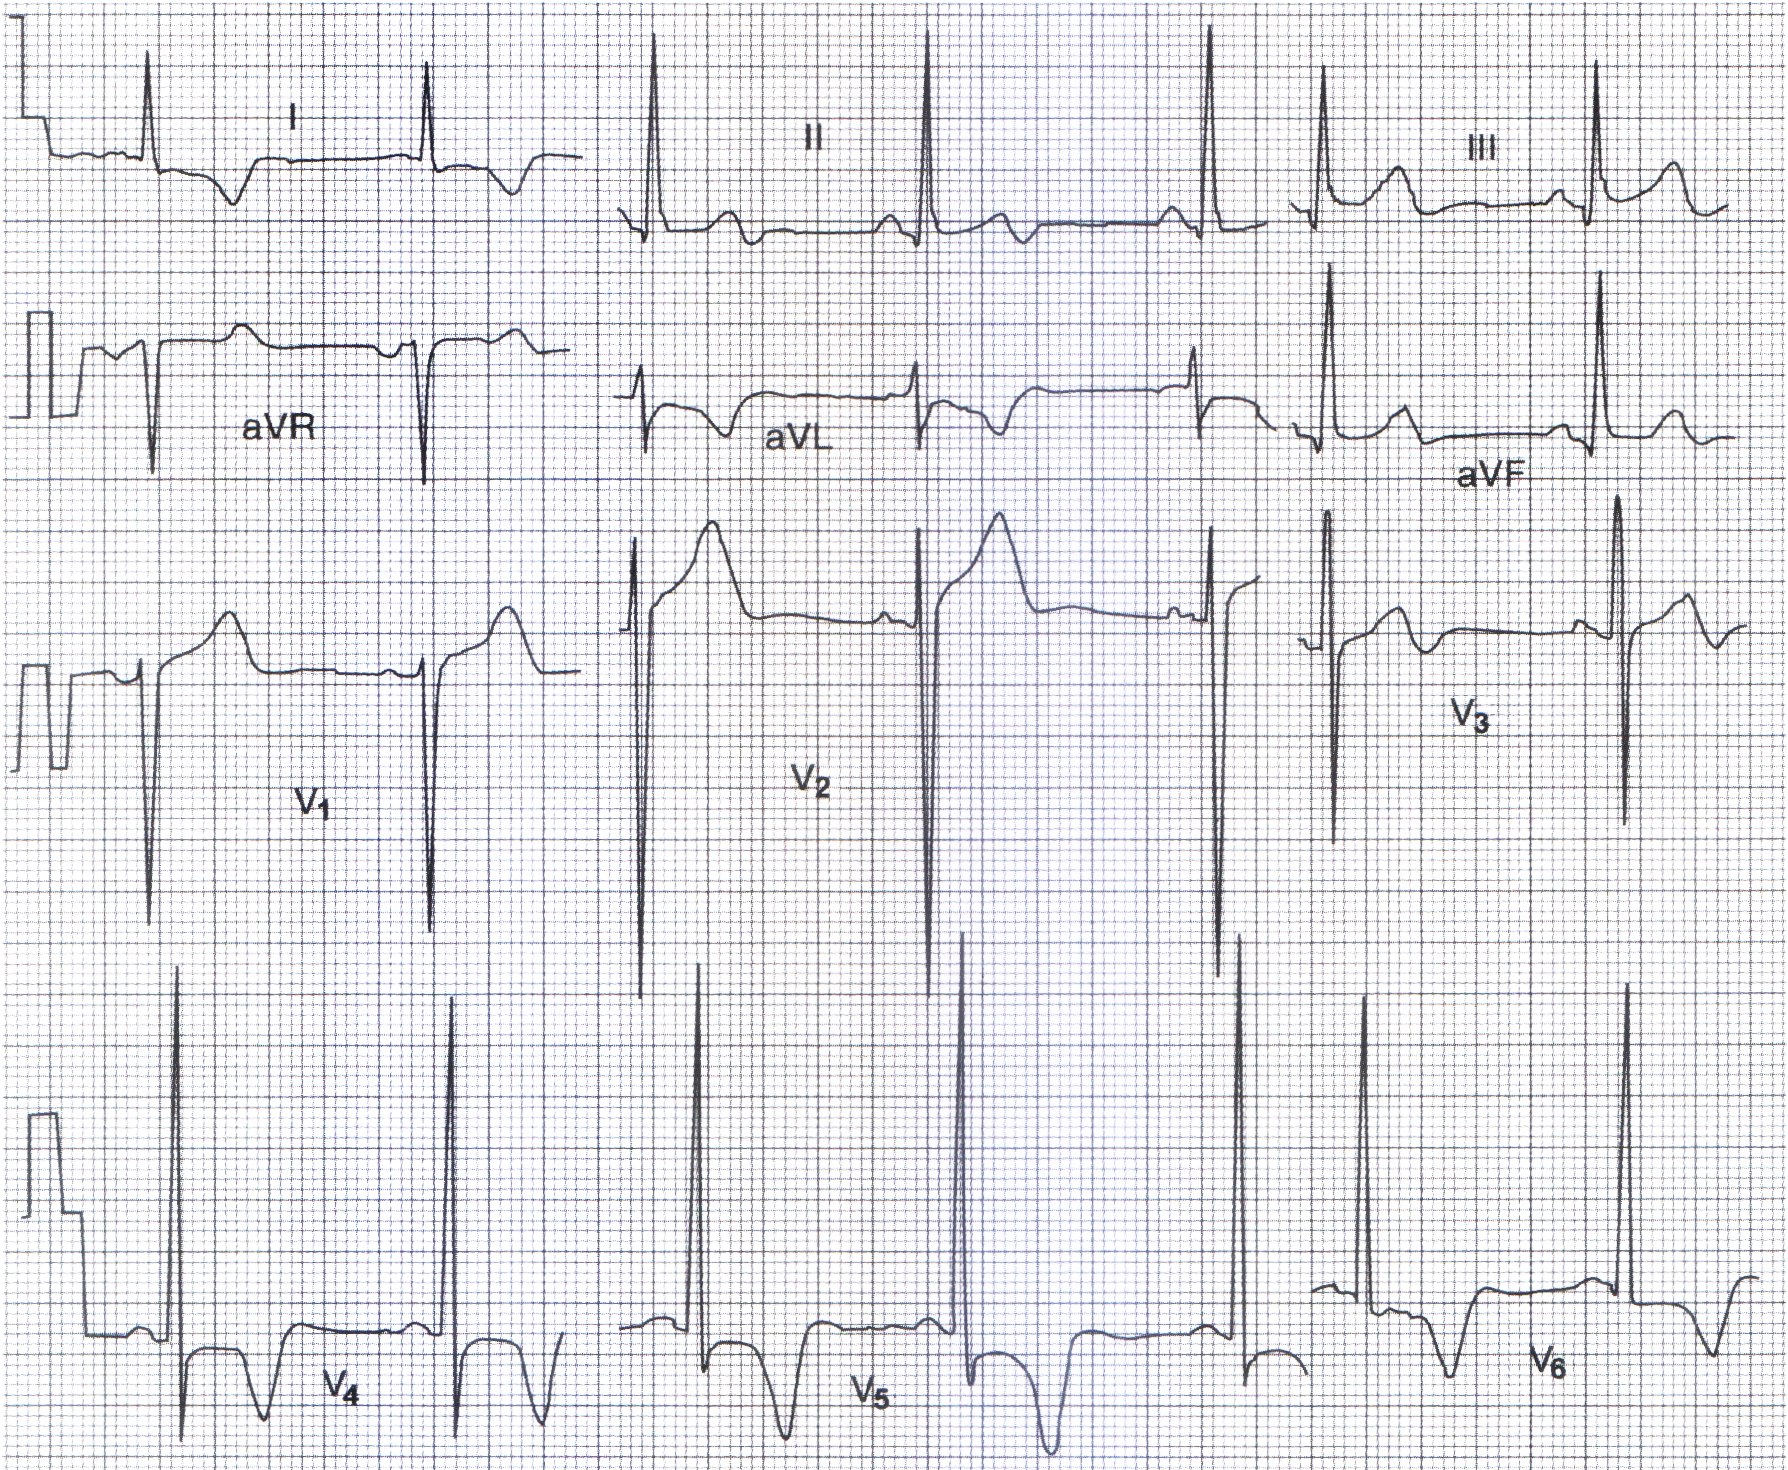
\includegraphics[scale=.9]{ecg-lvh.png}
			\centering \caption[Left ventricular hypertrophy]{Left ventricular hypertrophy \\$\bullet$ S in V\textsubscript{1} + R in V\textsubscript{6} or V\textsubscript{5} $>$35 mm (S V\textsubscript{1} + R V\textsubscript{6} $>$ 35 mm, for age $>$25 years);  \cite{abdullah-ecg}}
			\label{ecg-lvh}
		\end{figure}
		\item \textbf{RVH}: RAD + (R in V1 + S in V6) $>$ 11 mm
		\begin{figure}[htp]
			\centering \includegraphics[scale=.86]{ecg-rvh.png}
			\centering \caption[Right ventricular hypertrophy]{Right ventricular hypertrophy \\$\bullet$ Tall R wave in V\textsubscript{1} $>$7 mm (also deep S in V\textsubscript{5} or V\textsubscript{6}) \cite{abdullah-ecg}}
			\label{ecg-rvh}
		\end{figure}
	\end{enumerate}
\end{enumerate}

\newpage
\section{ST segment}\index{ST segment}
ST segment can me normal, elevated or depressed. 

\begin{enumerate}
	\item \textbf{ST elevation}\index{ST elevation}: Most commonly seen in \\
	-- Myocardial infarction \\
	-- Pericarditis 
	\begin{itemize}
		\item \textbf{Myocardial infarction}: $>$1 mm in chest leads, or, $>$2 mm in limb leads, in 2 or more leads. \\
		The affected leads show the area of infarct
		\begin{figure}[htp]
			\centering \includegraphics[scale=1.0]{ecg-ami.png}
			\centering \caption[Acute anterior MI]{Acute anterior MI (fully evolved case) \\$\bullet$ ST elevation (with upward convexity), Pathological Q wave, T inversion \cite{abdullah-ecg}}
			\label{ecg-acute-mi}
		\end{figure}
		\item \textbf{Pericarditis}: Usually all or most of the leads, with saddle shapped or concaved upwards. 
	\end{itemize}
	\item \textbf{ST depression}\index{ST depression}: It is a non-specific finding seen in \\
	-- Ischaemia\\
	-- Straing\\
	-- Contusion. 
\end{enumerate}

\section{T wave}\index{T wave}
The T wave can be normal or inverted. 

\noindent T inversion is a non-specific finding seen in, \\
-- Ischaemia \\
-- Other  

~\\
\noindent The classical pattern of myocardial infarction is, 
\begin{center}
	\begin{tabular}{r|l} 
		\toprule[1.5pt]
		%		& \textbf{LBBB} & \textbf{RBBB} \\ 
		%		\midrule
		ST elevation 	& minutes \\
		T inversion 	& hours \\
		Q wave 			& days \\
		%		\midrule
		%		\textit{Mnemonic} & \textit{WiLLiaM} & \textit{MoRRoW} \\
		\bottomrule[1.5pt]
	\end{tabular}
\end{center}


\section{Others}
\begin{itemize}
	\item \textbf{Sinus arrhythmias}\index{Sinus arrhythmias}
	\begin{enumerate}
		\item \textbf{Sinus arrhythmia}: Pulse rate varies with inspiration and expiration, \\
		-- \textit{Inspiration} sucks blood into heart, therefore to accommodate \textit{rate increases} \\
		-- \textit{Expiration} slows blood into heart, therefore to accommodate \textit{rate decreases} 
		\item \textbf{Sinus bradycardia}\index{Sinus bradycardia} ($<$60 bpm)\\
		-- Normal in athletes and elderly \\
		-- Secondary to hypothyroidism, hypothermia, cholestatic jaundice and $\uparrow$ ICP \\
		-- Drugs: $\beta$-blocker, digoxin
		-- Ischaemic heart disease affecting sinus node \\
		-- Degenerative disease of the sinus node \\
		\textbf{R\textsubscript{x}} of cause: Acutely -- IV Atropine, may need pacemaker  
		\item \textbf{Sinus tachycardia}\index{Sinus tachycardia} ($>$100 bpm) \\
		-- Physiological: Fever, exercise, emotion, pregnancy, anemia \\
		-- Pathological: Hyperthyroidism, raised catecholamines \\
		\textbf{R\textsubscript{x}} of cause: $\beta$-blockers
	\end{enumerate}
	\item \textbf{Pathological bradycardias} \\
	Physiologically, the pacemaker resides within SA node. Electrical impulses passes to the AV node, and then along the His-Purkinjie system to the rest of the heart. The SA node and AV node are supplied about 90\% and 60\% respectively by the right coronary artery. 
	\begin{enumerate}
		\item \textbf{Problems with the SA node (Sick Sinus Syndrome)}\index{Sick Sinus Syndrome}:\\
		-- Caused by ischaemic heart disease or, degenerative changes \\
		-- PR interval is prolonged to 2 sec \\
		-- May result in fast escape rhythms \\
		\textbf{R\textsubscript{x}}: Pacemaker, anticoagulation (thrombo-embolism is common in tachy-brady syndrome)
		
		\item \textbf{Problems with the AV node}: \\
		Please see the section of heart block syndrome (i.e. long PR interval)
%		\begin{enumerate}
%			\item \textbf{\ang{1} heart block} \\
%			-- Prolonged PR interval only 
%			\item \textbf{\ang{2} heart block} 
%			\begin{enumerate}
%				\item \textbf{Mobitz type I (Wenkebach)} \\
%				-- Increasing prolongation of PR interval followed by a dropped beat \\
%				-- This rhythm is usually benign, and needs no treatment 
%				\item \textbf{Mobitz type II}\\
%				-- Dropped beat with no previous prolongation of PR interval \\
%				-- May proceed to complete heart block, usually needs pacing 
%				\item \textbf{Advanced AV block} \\
%				-- Regular number of P waves per QRS, e.g. 2:1, 3:1, and so on. \\
%				-- May proceed to complete heart block, usually needs pacing 
%			\end{enumerate}
%			\item \textbf{Complete (\ang{3}) heart block}\\
%			-- No relationship between QRS and P waves \\
%			-- The QRS complexes are an escape rhythm, which could be either narrow ($<$3 small sq) or broad ($>$3 small sq)
%			\begin{enumerate}
%				\item \textbf{Narrow complex escape rhythm} \\
%				$\bullet$ Caused by block of AV node or a proximal block of the bundle of His \\
%				$\bullet$ This kind of escape rhythm is usually 50 -- 60 bpm, i.e. adequate \\
%				$\bullet$ Etiology could be the following,
%				\begin{itemize}
%					\item Congenital
%					\item Ischaemic heart disease (acute or chronic)
%					\item Diphtheria, Rheumatic fever
%					\item Digoxin toxicity, excess $\beta$-blockade 
%					\item Aortic calcification 
%					\item Endocarditis 
%				\end{itemize}
%				\textbf{R\textsubscript{x}} of cause, otherwise may not be necessary
%				\begin{itemize}
%					\item In acute case, atropine
%					\item Pacemaker if symptomatic
%					\item Many units pace even without symptoms
%				\end{itemize}
%				\item \textbf{Broad comeplex escape rhythm} \\
%				$\bullet$ Block is low down in His-Purkinjie system \\
%				$\bullet$ Escape rhythm is usually slow (15 -- 45 bpm) with dizziness and blackouts (Stock-Adams attack) \\
%				$\bullet$ In old age, usually due to degeneration of the His-Purkinjie system with calcification \\
%				-- Proximally -- Lenegre's disease \\
%				-- Distally -- Lev's disease \\
%				$\bullet$ In young patients, usually due to ischaemic heart disease \\
%				\textbf{R\textsubscript{x}}: All need pacemaker 
%			\end{enumerate}
%		\end{enumerate}
	\end{enumerate}
\end{itemize}


%========================
%	CHAPTER: OTHERS
%========================
\chapter{Others}

\section[Diet Calorie Values]{Calorie value of diets}\index{Calorie value}
\begin{table}[ht]
	\centering
	\caption{Calorie value of different diets}
	\begin{tabular}{r|l|r} 
		\toprule[1.5pt]
		& \textbf{Diet}	& \textbf{Calorie} \\ 
		\midrule
		1 & Milk suji 		& 67 Kcal/100 ml \\
		%		\midrule
		2 & Milk suji 100	& 100 Kcal/100 ml \\
		\midrule
		3 & Infant formula	& 68 Kcal/100 ml \\
		\midrule
		4 & \nicefrac{3}{4} rice suji	& 56.6 Kcal/100 ml \\
		%		\midrule
		5 & Full strength rice suji	& 70 Kcal/100 ml\\
		\midrule
		6 & Full strength biomil soya	& 68 Kcal/100 ml\\
		%		\midrule
		7 & \nicefrac{3}{4} strength biomil soya & 51 Kcal/100 ml\\
		\midrule
		8 & Full strength comminuted chicken & 60.6 Kcal/100 ml\\
		%		\midrule
		9 & \nicefrac{3}{4} strength comminuted chicken & 46.3 Kcal/100 ml\\
		\midrule
		%10 & Special milk & 100 Kcal/100 ml\\
		%		\midrule
		10 & Breast milk & 65 Kcal/100 ml\\
		\midrule
		11 & Chicken corn soup & 62 Kcal/100 ml\\
		\midrule
		12 & Khichuri & 145 Kcal/100 gm\\
		13 & Halwa & 240 Kcal/100 gm\\
		\midrule
		14 & Full strength pregistimil & 67 Kcal/100 ml\\
		%		\midrule
		15 & \nicefrac{3}{4} strength pregistimil & 50 Kcal/100 ml\\
		\bottomrule[1.5pt]
	\end{tabular}
	\begin{flushleft} 
		% Table notes.
	\end{flushleft}
	\label{Calorie}
\end{table}


\newpage
\section{Persistent Diarrhea}\index{Persistent Diarrhea}\index{PD}
\subsection{Definition}
Persistent diarrhoea is diarrhoea, with or without blood, that begins acutely and lasts for $\geq$14 days. \cite{islam2018management} 

\subsection{Dietary treatment algorithm}
\begin{figure}[htp]
	\centering \includegraphics[scale=0.22]{pd_algorithm.png}
	\centering \caption[PD treatment algorithm]{Treatment algorithm of icddr,b for children with persistent diarrhoea. \cite{islam2018management}}
	\label{PD}
\end{figure}

%\begin{enumerate}
%	\item Begin with, \begin{enumerate}
%		\item Age $<$ 6 months
%		\begin{enumerate}
%			\item Infant formula (low lactose), \\
%			if no response, \\
%			$\Downarrow$
%			\item Soy based formula (lactose and sucrose free diet)
%		\end{enumerate}
%		\item Age $\geq$ 6 months  
%		\begin{enumerate}
%			\item Milk Suji (Low lactose), \\
%			if no response, \\
%			$\Downarrow$
%			\item Rice suji
%			(lactose and sucrose free diet, mixture of rice powder, sugar \& oil),
%		\end{enumerate}
%	\end{enumerate} if treatment failure\textsuperscript{$\dagger$}, \\
%	$\Downarrow$
%	\item Comminuted Chicken (lactose, sucrose and maltose free diet), \\
%	if treatment failure, \\
%	$\Downarrow$
%	\item Hypoallergenic semi-elemental diet
%\end{enumerate}

\noindent {\color{red}$\star\star$} Treatment failure: \\
$\circ$ If deterioration of diarrhea, change to next diet after 3 days,\\
$\circ$ If remains static, change to next diet after 5--7 days. \\

\noindent {\color{red}$\star$} In case of improvement, back to previous diet after 5--7 days. 

\subsection{Plan of investigations}
\begin{enumerate}
	\item \textbf{\nth{1} line}: (Routine)
	\begin{enumerate}
		\item Complete Blood Count (CBC)
		\item Stool for Routine Microscopic Examination  
		\item Stool for culture for \textit{Salmonella, Shigella, Campylobacter jejuni, Vibrio cholerae, Aeromonas}
	\end{enumerate}
	\item \textbf{\nth{2} line}: (if high probality)
	\begin{enumerate}
		\item \textit{Cryptosporidium} by  ELISA
		\item \textit{Giardia} by ELISA
	\end{enumerate}
	\item \textbf{Associated investigations}:
	\begin{enumerate}
		\item Urine R/M/E
		\item Serum Electrolyte, Creatinine
		\item Chest radiograph
		\item Stool pH , electrolyte and Osmolality
		\item Stool for Sudan III stain
		\item Blood for C/S (if fever and sepsis is suspected)
		\item Others investigations according to patient status
	\end{enumerate}
	\item \textbf{In case of Chronic diarrhea}:
	\begin{enumerate}[noitemsep]
		\item Investigations to be given for PD (persistent diarrhea) \\+
		\item CBC (complete blood count) with PBF (peripheral blood film)
	\end{enumerate}
\end{enumerate}

\subsection{Management outline}
\begin{enumerate}
	\item \textbf{Proper counseling and } active participation of the parents or care giver
	\item \textbf{Rehydration}
	\begin{itemize}
		\item ORS in ``some'' or ``no'' dehydration
		\item IV fluid in ``severe'' dehydration or in ``some'' dehydration associated with frequent vomiting
	\end{itemize}
	\item \textbf{Infection identification and early intervention}
	\begin{itemize}
		\item Isolation of microorganism from stool examination
		\item Presence of any associated infection, e.g. UTI, pneumonia, CSOM etc.
	\end{itemize}
	\item \textbf{Dietary treatment}
	\begin{itemize}
		\item Reduce osmotic load
		\item Changing diet based on dietary (e.g. carbohydrate, fat etc.) malabsorption (Dietary Algorithm*)
	\end{itemize}
	\item \textbf{Treatment of complication}
	\begin{itemize}
		\item Electrolyte imbalance
		\item Hospital acquired infection
		\item Renal Failure
	\end{itemize}
\end{enumerate}


\newpage
%===========================
% 	BSA CALCULATION 
%===========================
\section[BSA Calculation]{Simplified calculation of BSA}\index{BSA}
\subsection{Height and weight known}
\[BSA = \sqrt{\frac{ht(cm) \times wt(kg)}{3600} } \]

Therefore, if weight is 7 kg and height is 70 cm, then BSA will be, \\\\
$= \sqrt{(70 \times 7) \bigg/ 3600} $ m\textsuperscript{2}\\
%$= \sqrt{490 \bigg/ 3600} $ m\textsuperscript{2}\\
%$= \sqrt{~0.136} $ m\textsuperscript{2}\\
$= 0.36878177829 $ m\textsuperscript{2}\\

\subsection{Weight known, height unknown}
\[BSA = {\frac{(wt \times 4) + 7}{wt + 90} } m^2 \]

% old styled formula writing: 
% \begin{equation}
%	BSA=\frac{(wt \times 4) + 7}{wt + 90} \text{m\textsuperscript{2}}
% \end{equation}\\

So, if wt is weight is 7 kg, then BSA will be, \\\\
$BSA = (7 \times 4) + 7 \bigg/ (7 + 90)$ m\textsuperscript{2}\\
$= (7 \times 4) + 7 \bigg/ (7 + 90)$ m\textsuperscript{2}\\
%$= 28 + 7 \bigg/ 97$ m\textsuperscript{2}\\
%$= 35 \bigg/ 97$ m\textsuperscript{2}\\
$= ~0.36082474226804123711$ m\textsuperscript{2}


\newpage
\section[Admission Criteria]{Admission criteria}\index{Admission criteria}
\begin{enumerate}
	\item \textbf{ICU}:
	\begin{enumerate}
		\item Severe sepsis, septic shock 
		\item Requiring respiratory support, \\
		$\circ$ Invasive: mechanical ventilation in respiratory failure \\
		$\circ$ Non-invasive: bubble CPAP in hypoxemia and grunting respiration 
		\item Convulsion, disorientation, or coma
		\item Hypothermia ($<$35.5\si{\celsius})
		\item Hypoglycemia ($\geq$2 times)
		\item Gross abnormalities in laboratory findings
	\end{enumerate}
	\item \textbf{LSU}:
	\begin{enumerate}
		\item \textbf{General criteria}:
		\begin{itemize}
			\item Patient with diarrhea (with or without co-morbidities) staying in SSU for $>$96 hours, with no improvement (after consultation with senior physician)
			\item Non-diarrheal patients under different studies with support (cost) from respective studies 
			\item In the event with confusion please consult with senior physicians before admission
		\end{itemize}
		\item \textbf{Specific criteria}: 
		\begin{enumerate}
			\item Weight for Length Z-score $<$--3 SD
			\item Weight for Age Z-score $<$--4 SD
			\item Bipedal edema 
			\item Premature, or, small for date neonate with diarrhea and signs of clinical sepsis 
			\item Severe pneumonia 
			\item Evaluation of PTB
			\item Persistent and/or chronic diarrhea 
			\begin{enumerate}
				\item If diarrhea persists $\geq$14 days (after obtaining careful history) + signs of dehydration \\
				(in case of any confusion, please consult with senior physician)
				\item In case of PD (persistent diarrhea; duration $\geq$14 days), without any malnutrition or other illnesses, observe the patient for 2 days in SSU. If no improvement $\rightarrow$ admit in LSU 
				\item Chronic diarrhea ($>$4 weeks) with supporting documents 
			\end{enumerate}
			\item Clinical jaundice with co-morbidities and signs of dehydration
			\item Suspected electrolytes imbalance, except tetany
			\item Urinary suppression $\geq$24 hours, without dehydration (please take history and check for retention of urine)
			\item Moderate and severe acute asthma, acute exacerbation of COPD 
			\item Age $\geq$70 years, after consultation with senior physician
			\item NRU (Nutritional rehabilitation unit):
			\begin{itemize}
				\item Resolution of acute phase $+$
				\item Weight for Length Z-score $<$--3 SD
				\item Weight for Age Z-score $<$--4 SD
				\item Nutritional edema 
			\end{itemize}
		\end{enumerate}
	\end{enumerate}
\end{enumerate}


\newpage
%===============================
%	PHYSIOLOGICAL RANGES
%===============================
\section[Few Physiological Ranges]{Few physiological ranges}
%\subsection{Fast breathing ranges}
%\begin{table}[ht]
%	\centering
%	\caption{Age specific fast breathing in children}
%	\begin{tabular}{l|c}
%		\toprule[1.5pt]
%		Age 		& Breaths per minute \\
%		\midrule
%		$<$2 months		& $\geq$60 bpm \\
%		2 -- 11 months 	& $\geq$50 bpm \\
%		$>$1 year 		& $\geq$40 bpm \\ 
%		\bottomrule[1.5pt]
%	\end{tabular}
%	\begin{center} 
%		Taken from icddr,b Dhaka hospital protocol.
%	\end{center}
%	\label{RR}
%\end{table}

\subsection{Normal respiratory rates in infants and children}
\begin{table}[ht]
	\centering
	\caption{Ranges of RRs in children}
	\begin{tabular}{l|c}
		\toprule[1.5pt]
		Age 		& Breaths per minute \\
		\midrule
		Newborn -- 1 year	& 30 -- 60 bpm \\
		1 -- 2 years		& 24 -- 40 bpm \\
		2 -- 5 years 		& 22 -- 34 bpm \\
		6 -- 11 years 		& 18 -- 30 bpm \\
		$\geq$12 years 		& 12 -- 20 bpm \\
		\bottomrule[1.5pt]
	\end{tabular}
	\begin{center} 
		Taken from Childhood TB Portal, where normal temperature was regarded as $\leq$38\si{\celsius}  \cite{childhoodtb}.
	\end{center}
	\label{RR}
\end{table}

\subsection{Normal BP ranges in infants and children}
\begin{table}[ht]
	\centering
	\caption{Ranges of BPs in children}
	\begin{tabular}{l|c}
		\toprule[1.5pt]
		Age 		& Systolic BP (mmHg) \\
		\midrule
		premature 	& 55 - 65 \\
		0 - 3 m 	& 65 - 85 \\
		3 - 6 m 	& 70 - 90 \\
		6 - 12 m 	& 80 - 100 \\
		1 - 3 y 	& 90 - 105 \\
		3 - 6 y 	& 95 - 110 \\
		\bottomrule[1.5pt]
	\end{tabular}
	\begin{flushleft} 
		% Table notes.
	\end{flushleft}
	\label{Systolic BP}
\end{table}

~\\
\subsection{Pulse rate and BP ranges in children}
\begin{table}[ht]
	\centering
	\caption{Ranges of Pulse rate and BPs in children}
	\begin{tabular}{c|c|c} 
		\toprule[1.5pt]
		Age (years) 	& Pulse rate (range) 	& Systolic BP (mmHg) \\ 
		\midrule
		0 - 1 			& 100 - 160 			& \textgreater 60 \\ 
		1 - 3 			& 90 - 150 				& \textgreater 70 \\
		3 - 6	 		& 80 - 140 				& \textgreater 75 \\
		\bottomrule[1.5pt]
	\end{tabular}
	\begin{flushleft} 
		% Table notes.
	\end{flushleft}
	\label{Pulse BP}
\end{table}

\newpage
\section{TB in children}
\subsection{Diagnostic clinical criteria}
The presence of $\geq$3 of the following features, suggests a diagnosis of TB. 
\begin{enumerate}
	\item Symptoms suggestive of TB \index{TB}
	\item A history of recent close contact ($\leq$12 months)
	\item Physical signs highly suggestive of TB
	\item A positive Montoux test \index{Montoux test}
	\item Chest X-ray suggestive of TB
	\item Special laboratory tests, e.g. CSF examinations, histopathology
\end{enumerate}

\noindent{\color{red}\textbf{NB}}: If a child has only 2 features and other criteria are no helpful in diagnosis, expert opinion should be sought before proceeding further. 

\subsection[Key risk factors]{Key risk factors for TB in children}
\begin{enumerate}
	\item Household or close contact with a smear positive or culture positive pulmonary TB (e.g. parents, siblings, close relatives, neighbors, teachers). 
	\item Age $<$5 years: As the risk of developing TB is  highest in very young children, who is immune immature. 
	\item Severe malnutrition or other immunosuppressive conditions, 
	\begin{itemize}
		\item Measles in past 3 months 
		\item Whooping cough 
		\item HIV infection 
		\item Being on drugs like steroids, or other immunosuppressive agents 
	\end{itemize}
	\item The time since exposure or infection: The vast majority of children who develop TB, do so \textbf{within the first year} after \textit{M. tuberculosis} exposure or infection 
\end{enumerate}

\noindent{\color{red}\textbf{NB}}: Other risk factors are HIV/ AIDS, diabetes, end-stage renal failure, cancer, connective tissue disease, silicosis, gastrectomy, solid organ transplantation and patients on prolong steroids. Both type I and type II diabetic patients have the increased risk of having TB. 

%\newpage
%\section{Larynx and Pharynx}
%\begin{figure}[htp]
%	\centering \includegraphics[scale=0.66]{/home/pr33/MEGA/Documents/icddrb/icddrb-ICU-protocols/LaTeX/fig/larynx-pharynx.jpg}
%	\centering \caption[The larynx and pharynx]{A schematic diagram of laryx and pharynx \cite{larynxpharynx}}
%	\label{ECG}
%\end{figure}
%
%
%\section{The coverings of the brain}
%\begin{figure}[htp]
%	\centering \includegraphics[scale=0.495]{/home/pr33/MEGA/Documents/icddrb/icddrb-ICU-protocols/LaTeX/fig/layers-of-meninges-evan-oto.png}
%	\centering \caption[The brain coverings]{The dura mater, arachnoid mater and pia mater}
%	\label{braincerings}
%\end{figure}



%\section[Presenting Chest X-ray]{While presenting a Chest X-ray}
%${\color{red}\star\star\star}$ First, look for ``R'' or ``L'' to confirm the side.
%
%\begin{itemize}
%	\item \textbf{Presenting a normal chest X-ray}: 
%	CXR PA view showing: 
%	\begin{enumerate}
%		\item Lung fields are clear on both sides
%		\item Trachea is centrally placed
%		\item Both domes of diaphragm are normal in position
%		\item Costophrenic and cadiophrenic angles are clear on both sides 
%		\item The heart is normal in transverse diameter 
%		\item Bony configuration is normal
%	\end{enumerate}
%	\item However, \textbf{findings often get missed}: Be careful, when CXR appears to be apparently normal, or you are unable to see any finding. 
%	Look carefully and search for the following findings: 
%	\begin{enumerate}
%		\item Cervical rib (unilateral or bilateral, small or rudimentary)
%		\item Small apical pneumothorax 
%		\item Azygos lobe 
%		\begin{figure}[htp]
%			\centering \includegraphics[scale=0.18]{/home/pr33/MEGA/Documents/icddrb/icddrb-ICU-protocols/LaTeX/fig/kerleys-line-acute-pulmonary-oedema-azygos-lobe.png}
%			\centering \caption[Kerley's line and Azygos lobe]{Kerley's line and Azygos lobe \cite{azygoslobe, kerleysline}}
%			\label{Azygoslobe-Kerlysline}
%		\end{figure}
%		\item Kerley's line (B and A)
%		\item Bullae (may be small or large)
%		\item Rib notching 
%		\item Absent breast shadow in female (due to mastectomy)
%		\item Small pleural effusion 
%		\item Fluid level behind the heart (hiatus hernia, achalasia)
%		\item Subdiaphragmatic gas shadow 
%		\item Subcutaneous emphysema (in soft tissue of chest wall and neck)
%		\item Thickened trabeculae in the ribs, clavicle, scapula (in hereditary hemolytic anemia)
%	\end{enumerate}
%\end{itemize}
%Taken from Professor ABM Abdullah's Radiology in Medical Practice \cite{abdullahradiology}. 


\chapter{Further Reading}
\begin{enumerate}
	\item Guidelines for treatment of drug-susceptible tuberculosis and patient care, 
	2017, World Health Organization, 
	ISBN: 978-92-4-155000-0
	\item Pocketbook of hospital care for children, 
	\nth{2} edition, 2013, World Health Organization, 
	ISBN: 978 92 4 154837 3
	\item Revised WHO classification and treatment of childhood pneumonia at health facilities, 
	2014, World Health Organization, 
	ISBN: 978 92 4 150781 3
	\item Updates on the management of severe acute malnutrition in infants and children, 
	2013, World Health Organization, 
	ISBN: 978 92 4 150632 8
\end{enumerate}


%======================
%	BIOLIOGRAPHY
%======================
\addcontentsline{toc}{chapter}{Reference}
\bibliographystyle{IEEEtran}
\bibliography{handbook-reference.bib}

\printindex


\newpage
\clearpage
\begin{center}
	\thispagestyle{empty}
	\vspace*{\fill}
	{\huge \textbf{THE END}}
	\vspace*{\fill}
\end{center}
\clearpage


%---------------------
%	END OF THE LINE 
%---------------------
\end{document}